\part{圆}
\section{基本性质}
\begin{definition}[圆]
    在一个平面内,围绕一个定点$O$并以一定长度$r$为距离旋转一周所形成的封闭曲线叫做圆(Circle)。定点$O$称作圆心,$r$称作圆的半径。圆是到定点O的距离等于定长r的点的集合。\\
    (1) 半径: 连接圆心和圆上任意一点的线段叫做半径,字母表示为r。\\
    (2) 直径: 通过圆心并且两端都在圆上的线段叫做直径,字母表示为d。直径所在的直线是圆的对称轴。\\
    (3) 弦:连接圆上任意两点的线段叫做弦,在同一个圆内最长的弦是直径。\\
    (4) 弧: 圆上任意两点间的部分叫做圆弧,简称弧,符号表示为$\overset{\frown}{AB}$。大于半圆的弧称为优弧,例如$\overset{\frown}{ADB}$;小于半圆的弧称为劣弧,如$\overset{\frown}{AB}$。同一圆中能够互相重合的两条弧叫做等弧。\\
    (5) 任意定点及定长可以构成一个圆。圆心和半径同时相同的圆为同圆,圆心相同半径不同的圆称作同心圆,半径相同圆心不同的圆称作等圆。\\
\end{definition}

\begin{figure}[H]
    \centering
    \includegraphics[width=\linewidth]{figures/圆.png}
\end{figure}


\section{垂径定理}
\begin{theorem}[垂径定理]
圆具有旋转不变性以及对称性。垂直于弦的直径平分这条弦,且平分弦所对的两条弧。
\end{theorem}
\begin{figure}[H]
    \centering
    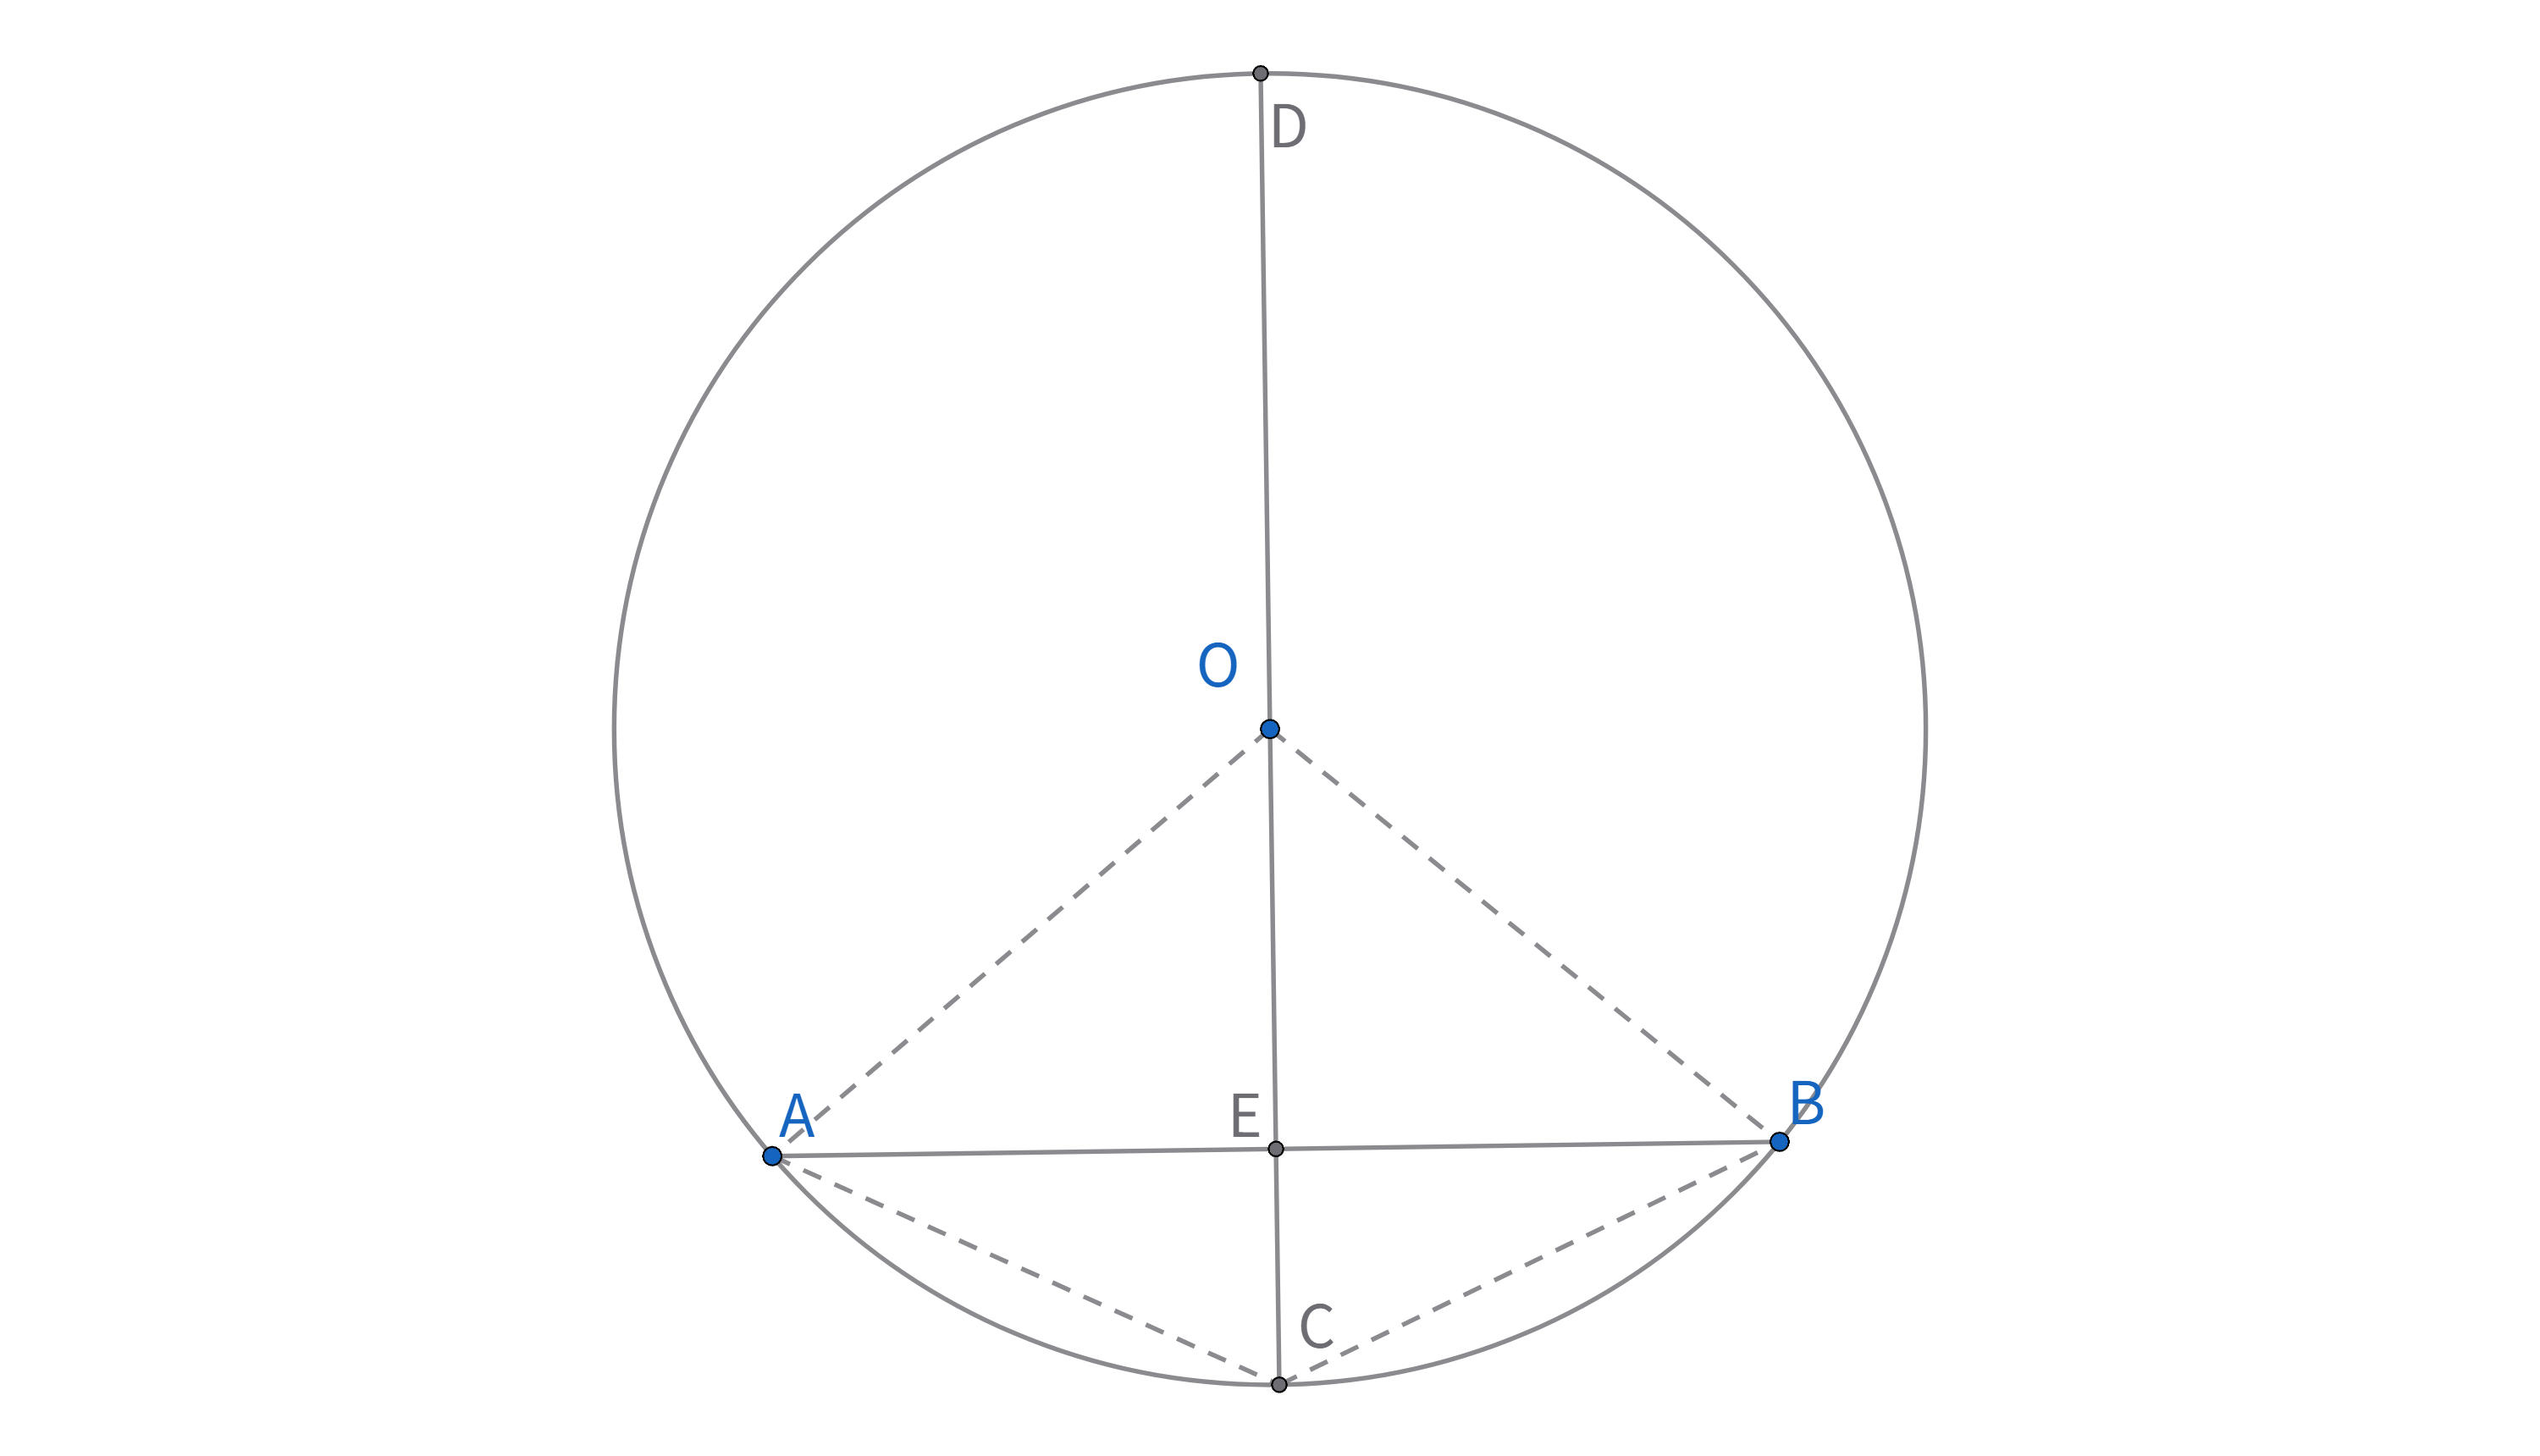
\includegraphics[width=\linewidth]{figures/垂径定理.png}
    \caption{垂径定理}
    % \label{fig:enter-label}
\end{figure}



\section{圆周角定理}
\begin{theorem}[圆周角定理]
    对任意一条弦,与圆心构成的顶角称作圆心角,与圆周上另一点构成的顶角叫做圆周角。圆内的圆周角具有如下性质:
    
    (1) 直径所对圆周角为90度。
    
    (2) 同弧所对圆周角度数是圆心角的一半。
    
    (3) 同弧或等弧所对圆周角度数相等。

    (4) 弦分割的两圆弧所对圆周角互补。
\end{theorem}
\begin{figure}[H]
    \centering
    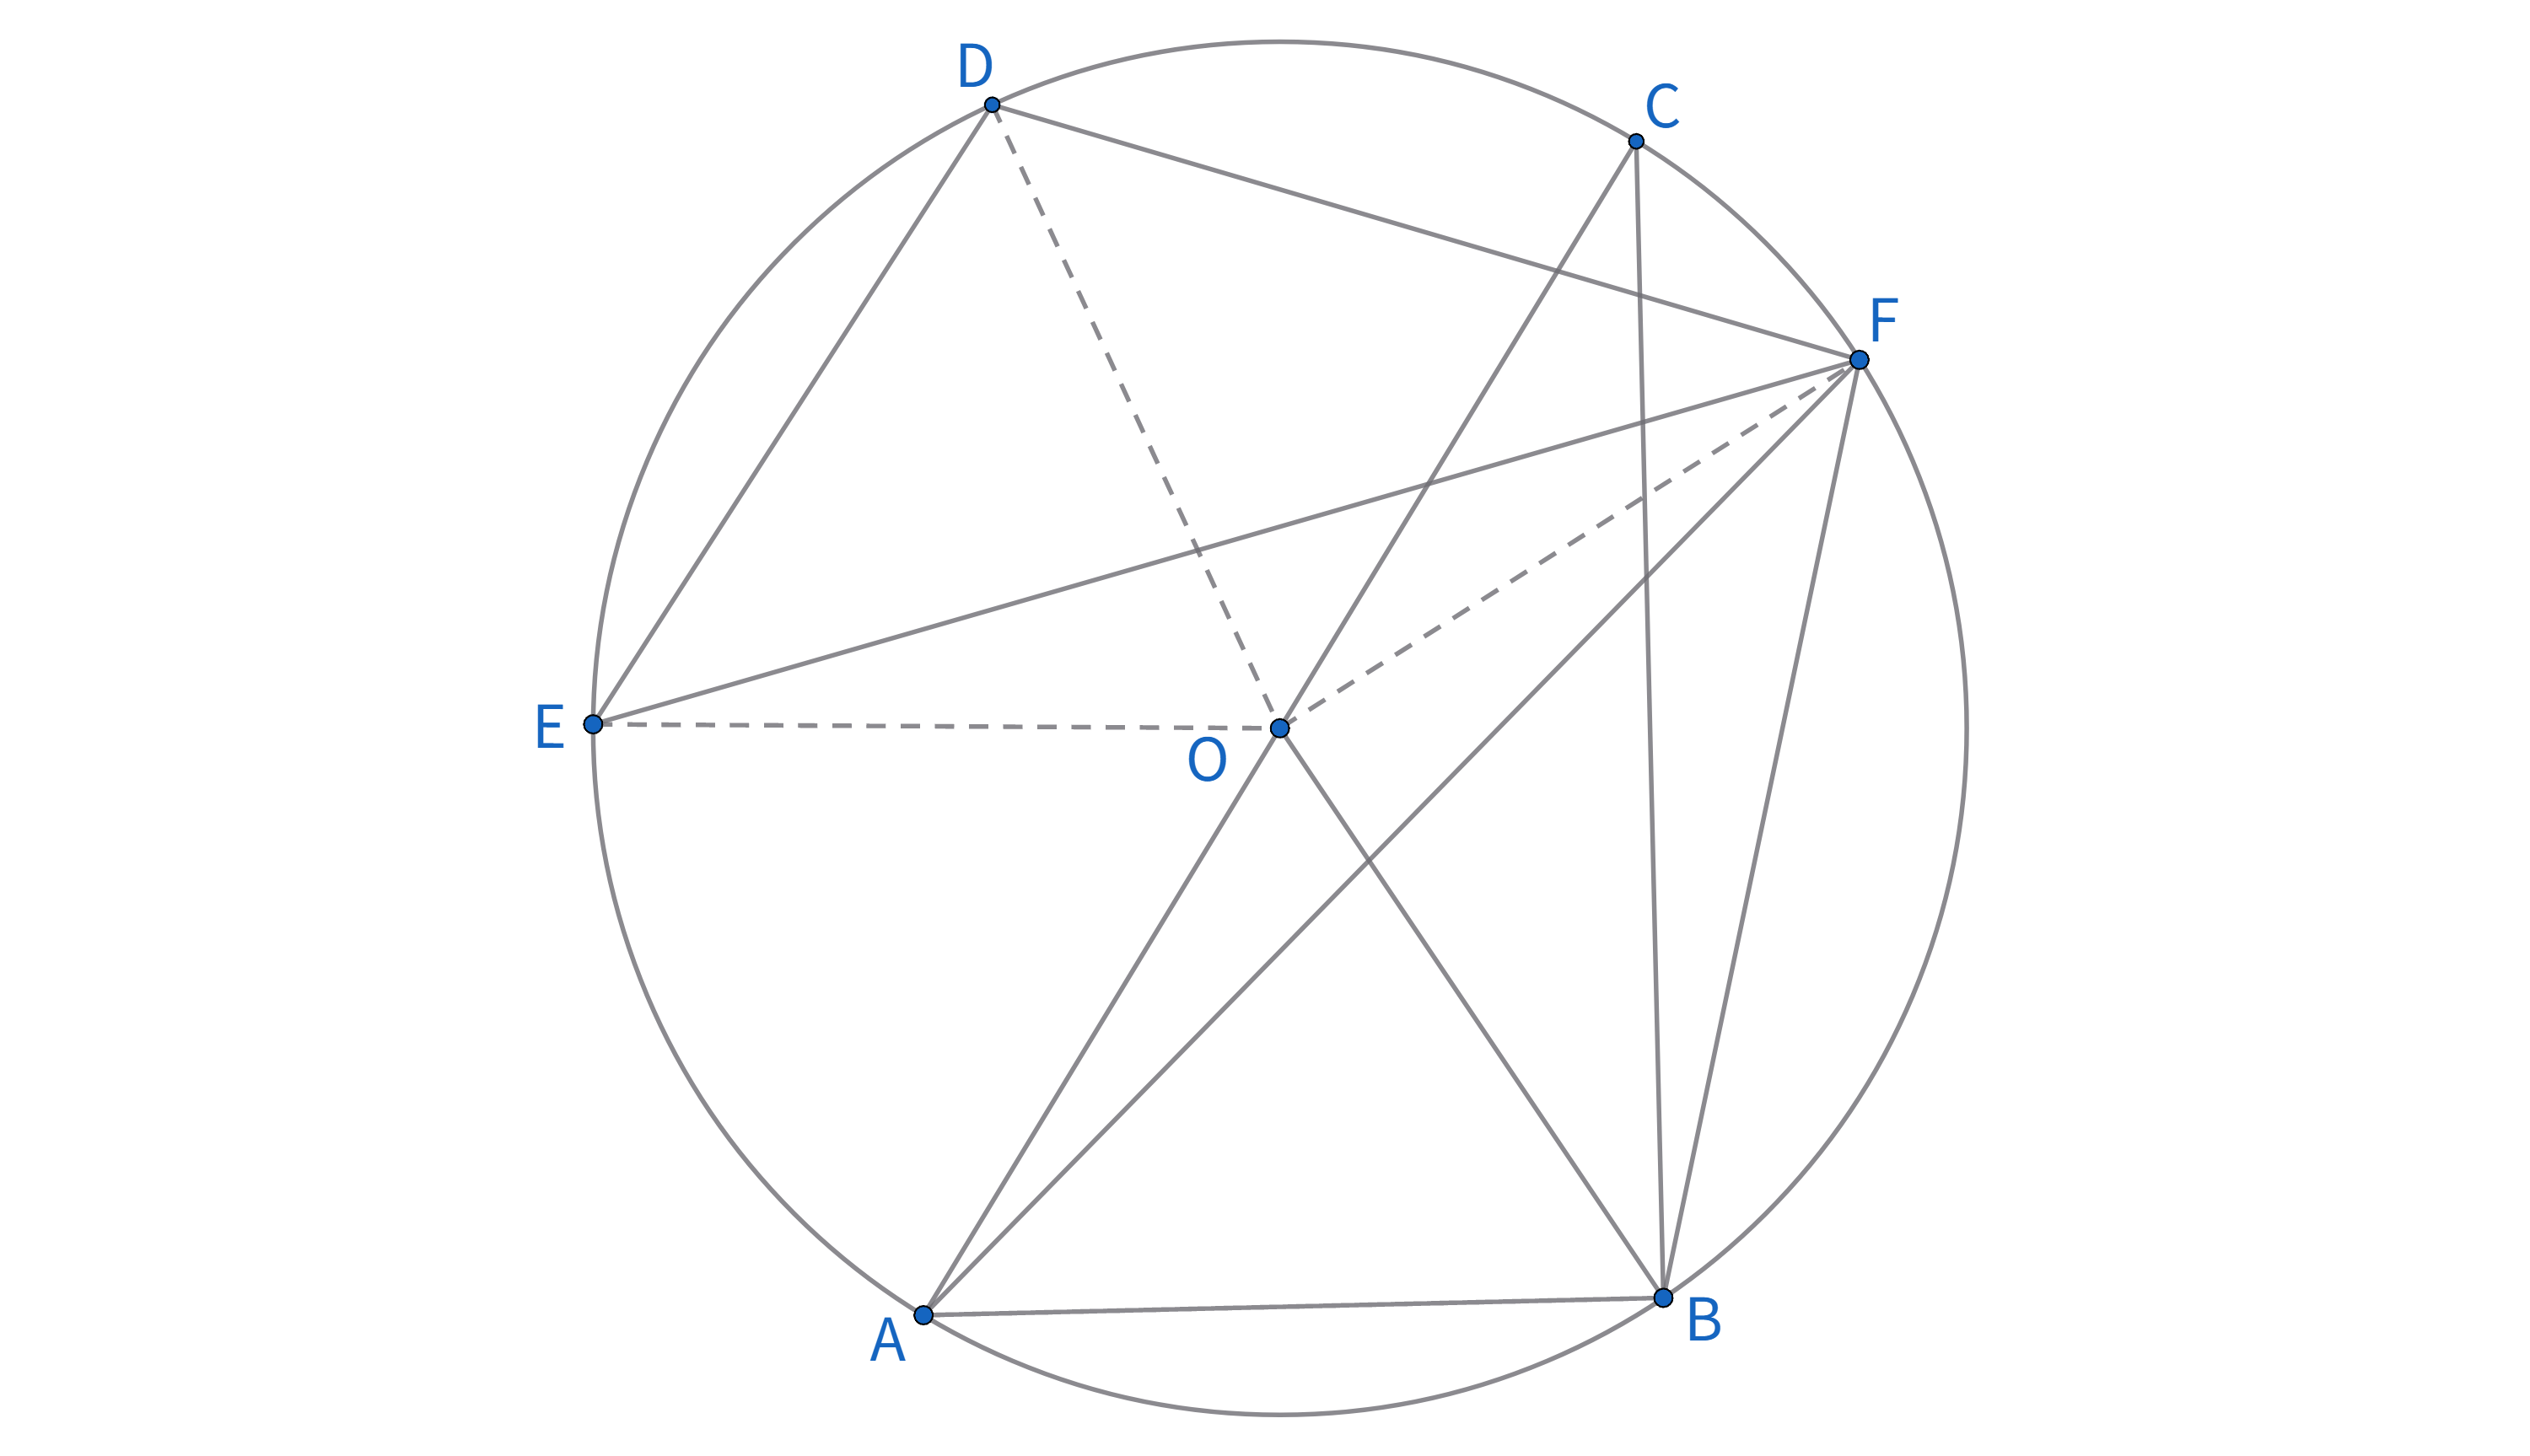
\includegraphics[width=0.8\linewidth]{figures/圆周角定理.png}
    \caption{圆周角定理}
    % \label{fig:enter-label}
\end{figure}
\begin{figure}[H]
    \centering
    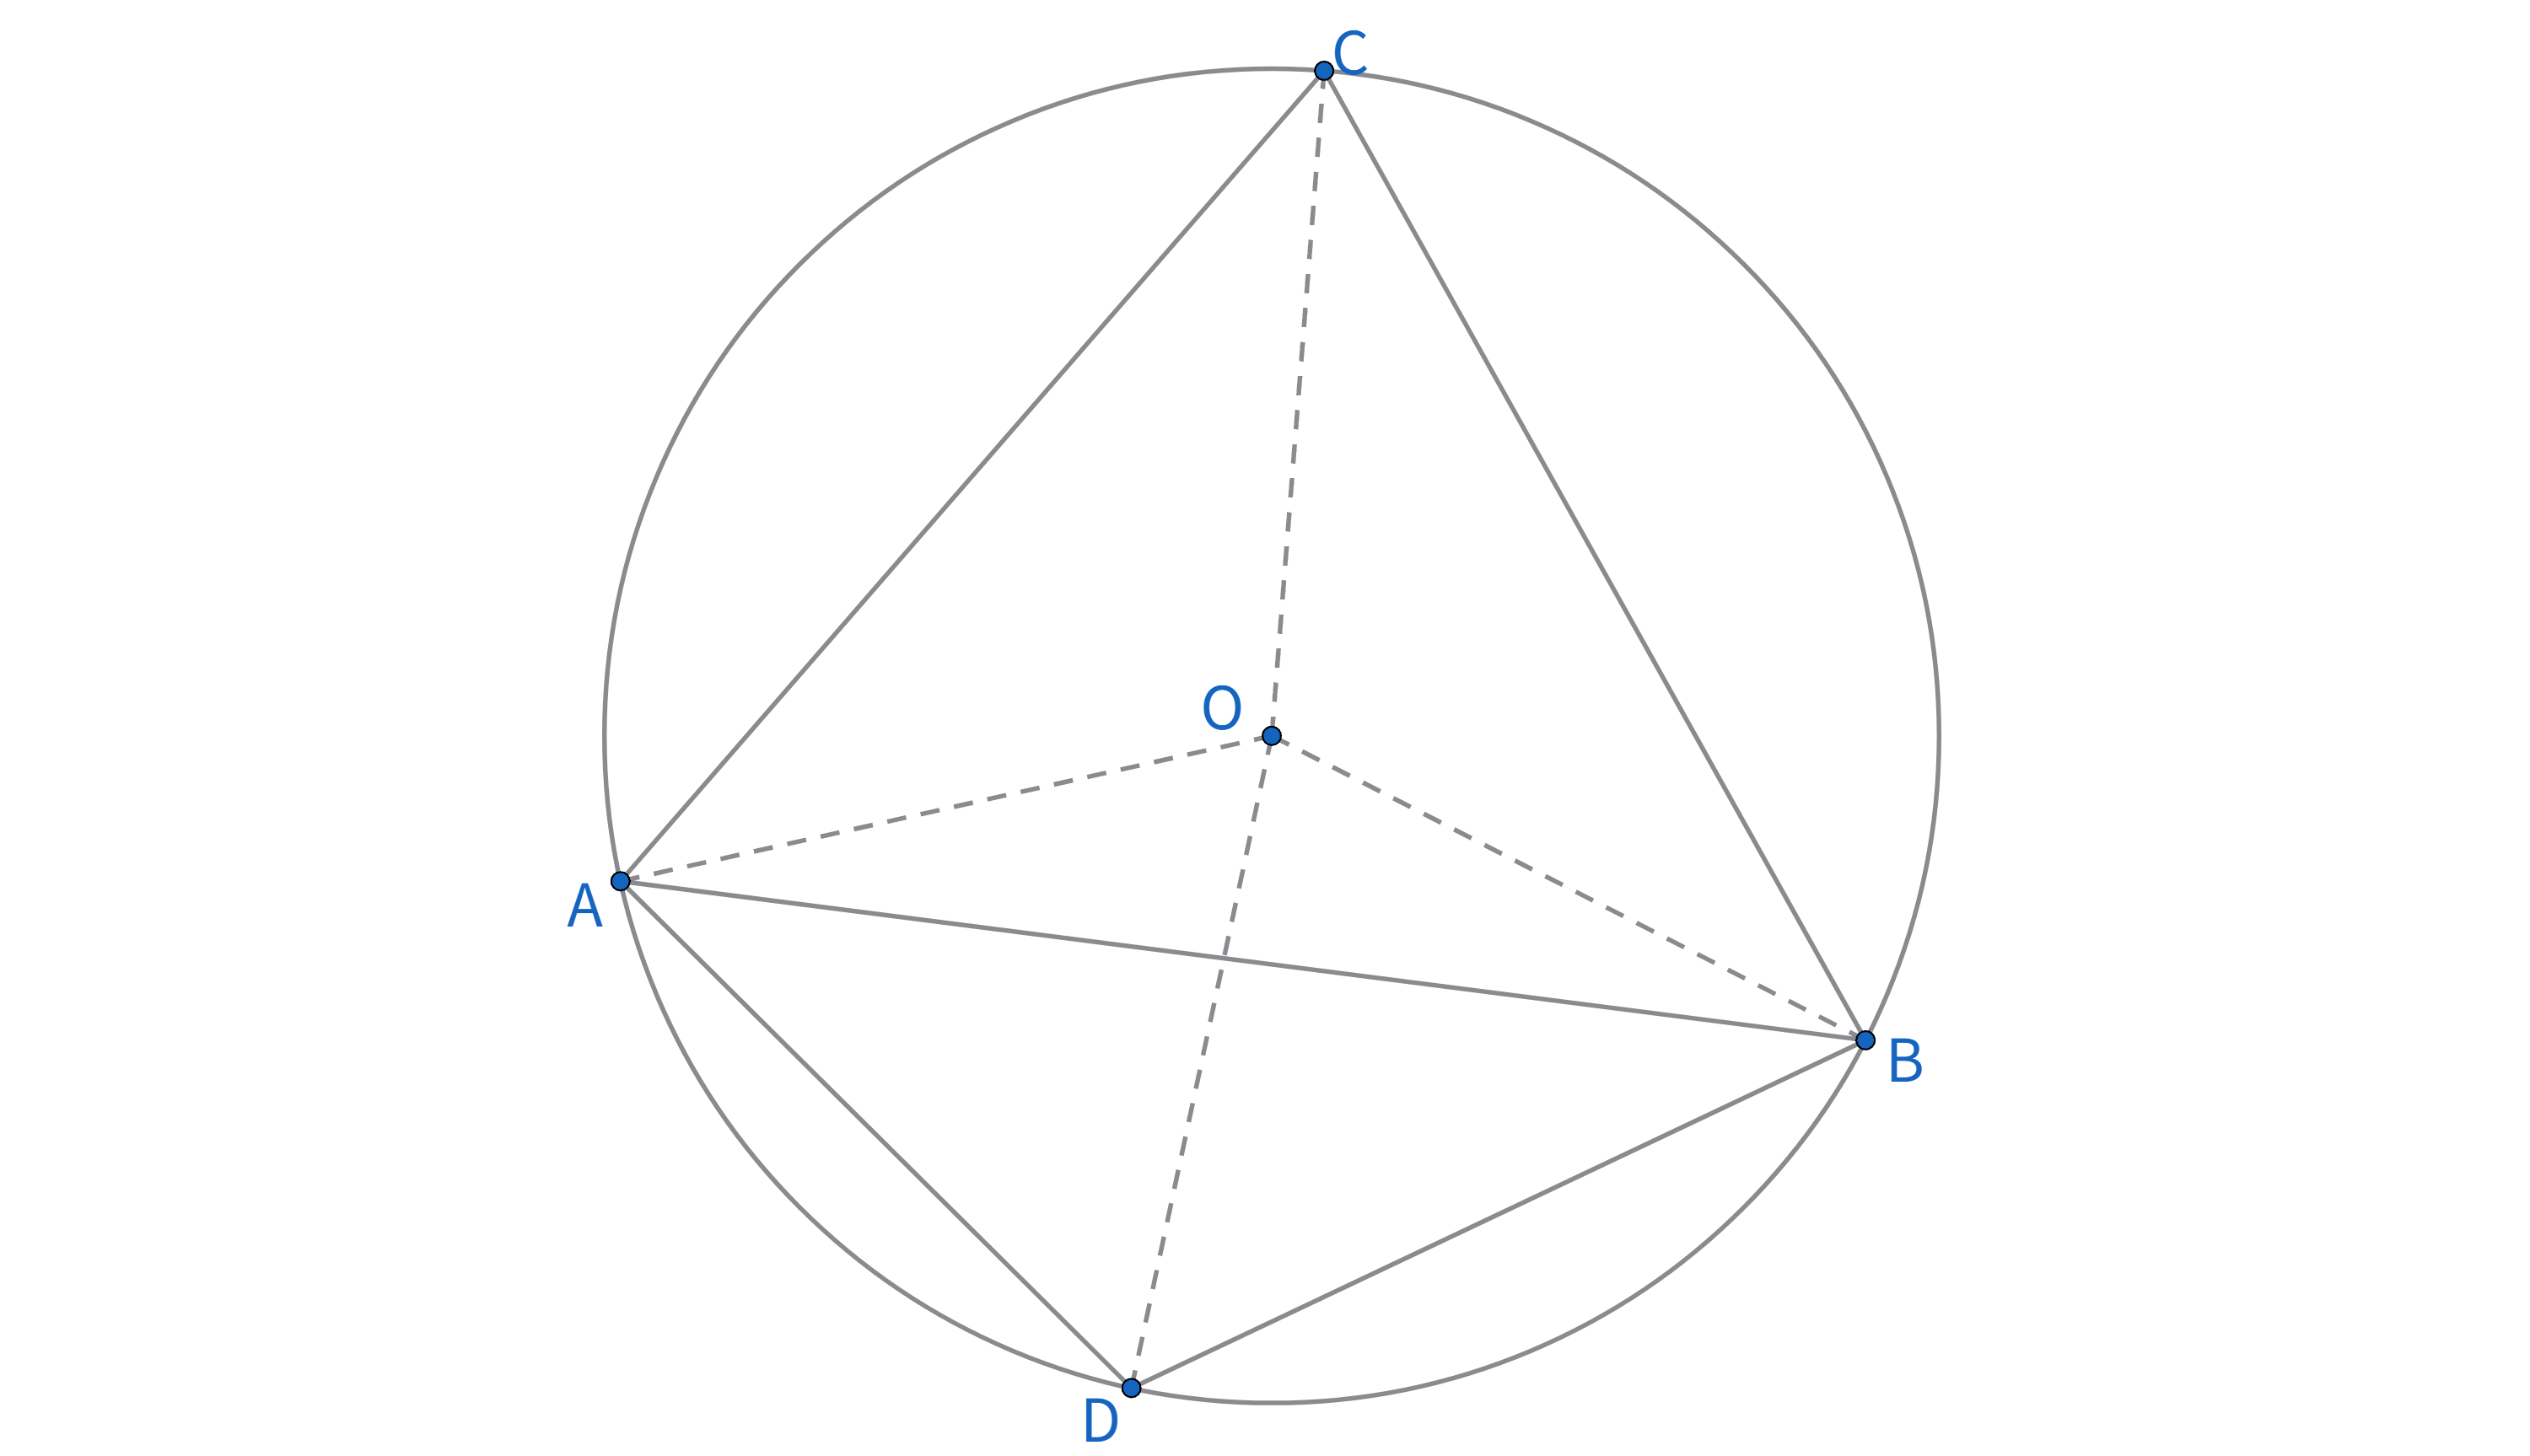
\includegraphics[width=0.8\linewidth]{figures/圆周角定理-对角互补.png}
    \caption{对角互补}
    % \label{fig:enter-label}
\end{figure}



\section{点与圆的位置关系}
用$d(A,B)$表示两点A和B的距离,点与圆的关系可分为三类。
\begin{itemize}
    \item 点在圆外:当点A与圆心O的距离大于半径r时,即$d(A,O) > r$。
    \item 点在圆上:当点A与圆心O的距离等于半径r时,即$d(A,O) = r$。
    \item 点在圆内:当点A与圆心O的距离小于半径r时,即$d(A,O) < r$。
\end{itemize}
\begin{figure}[H]
    \centering
    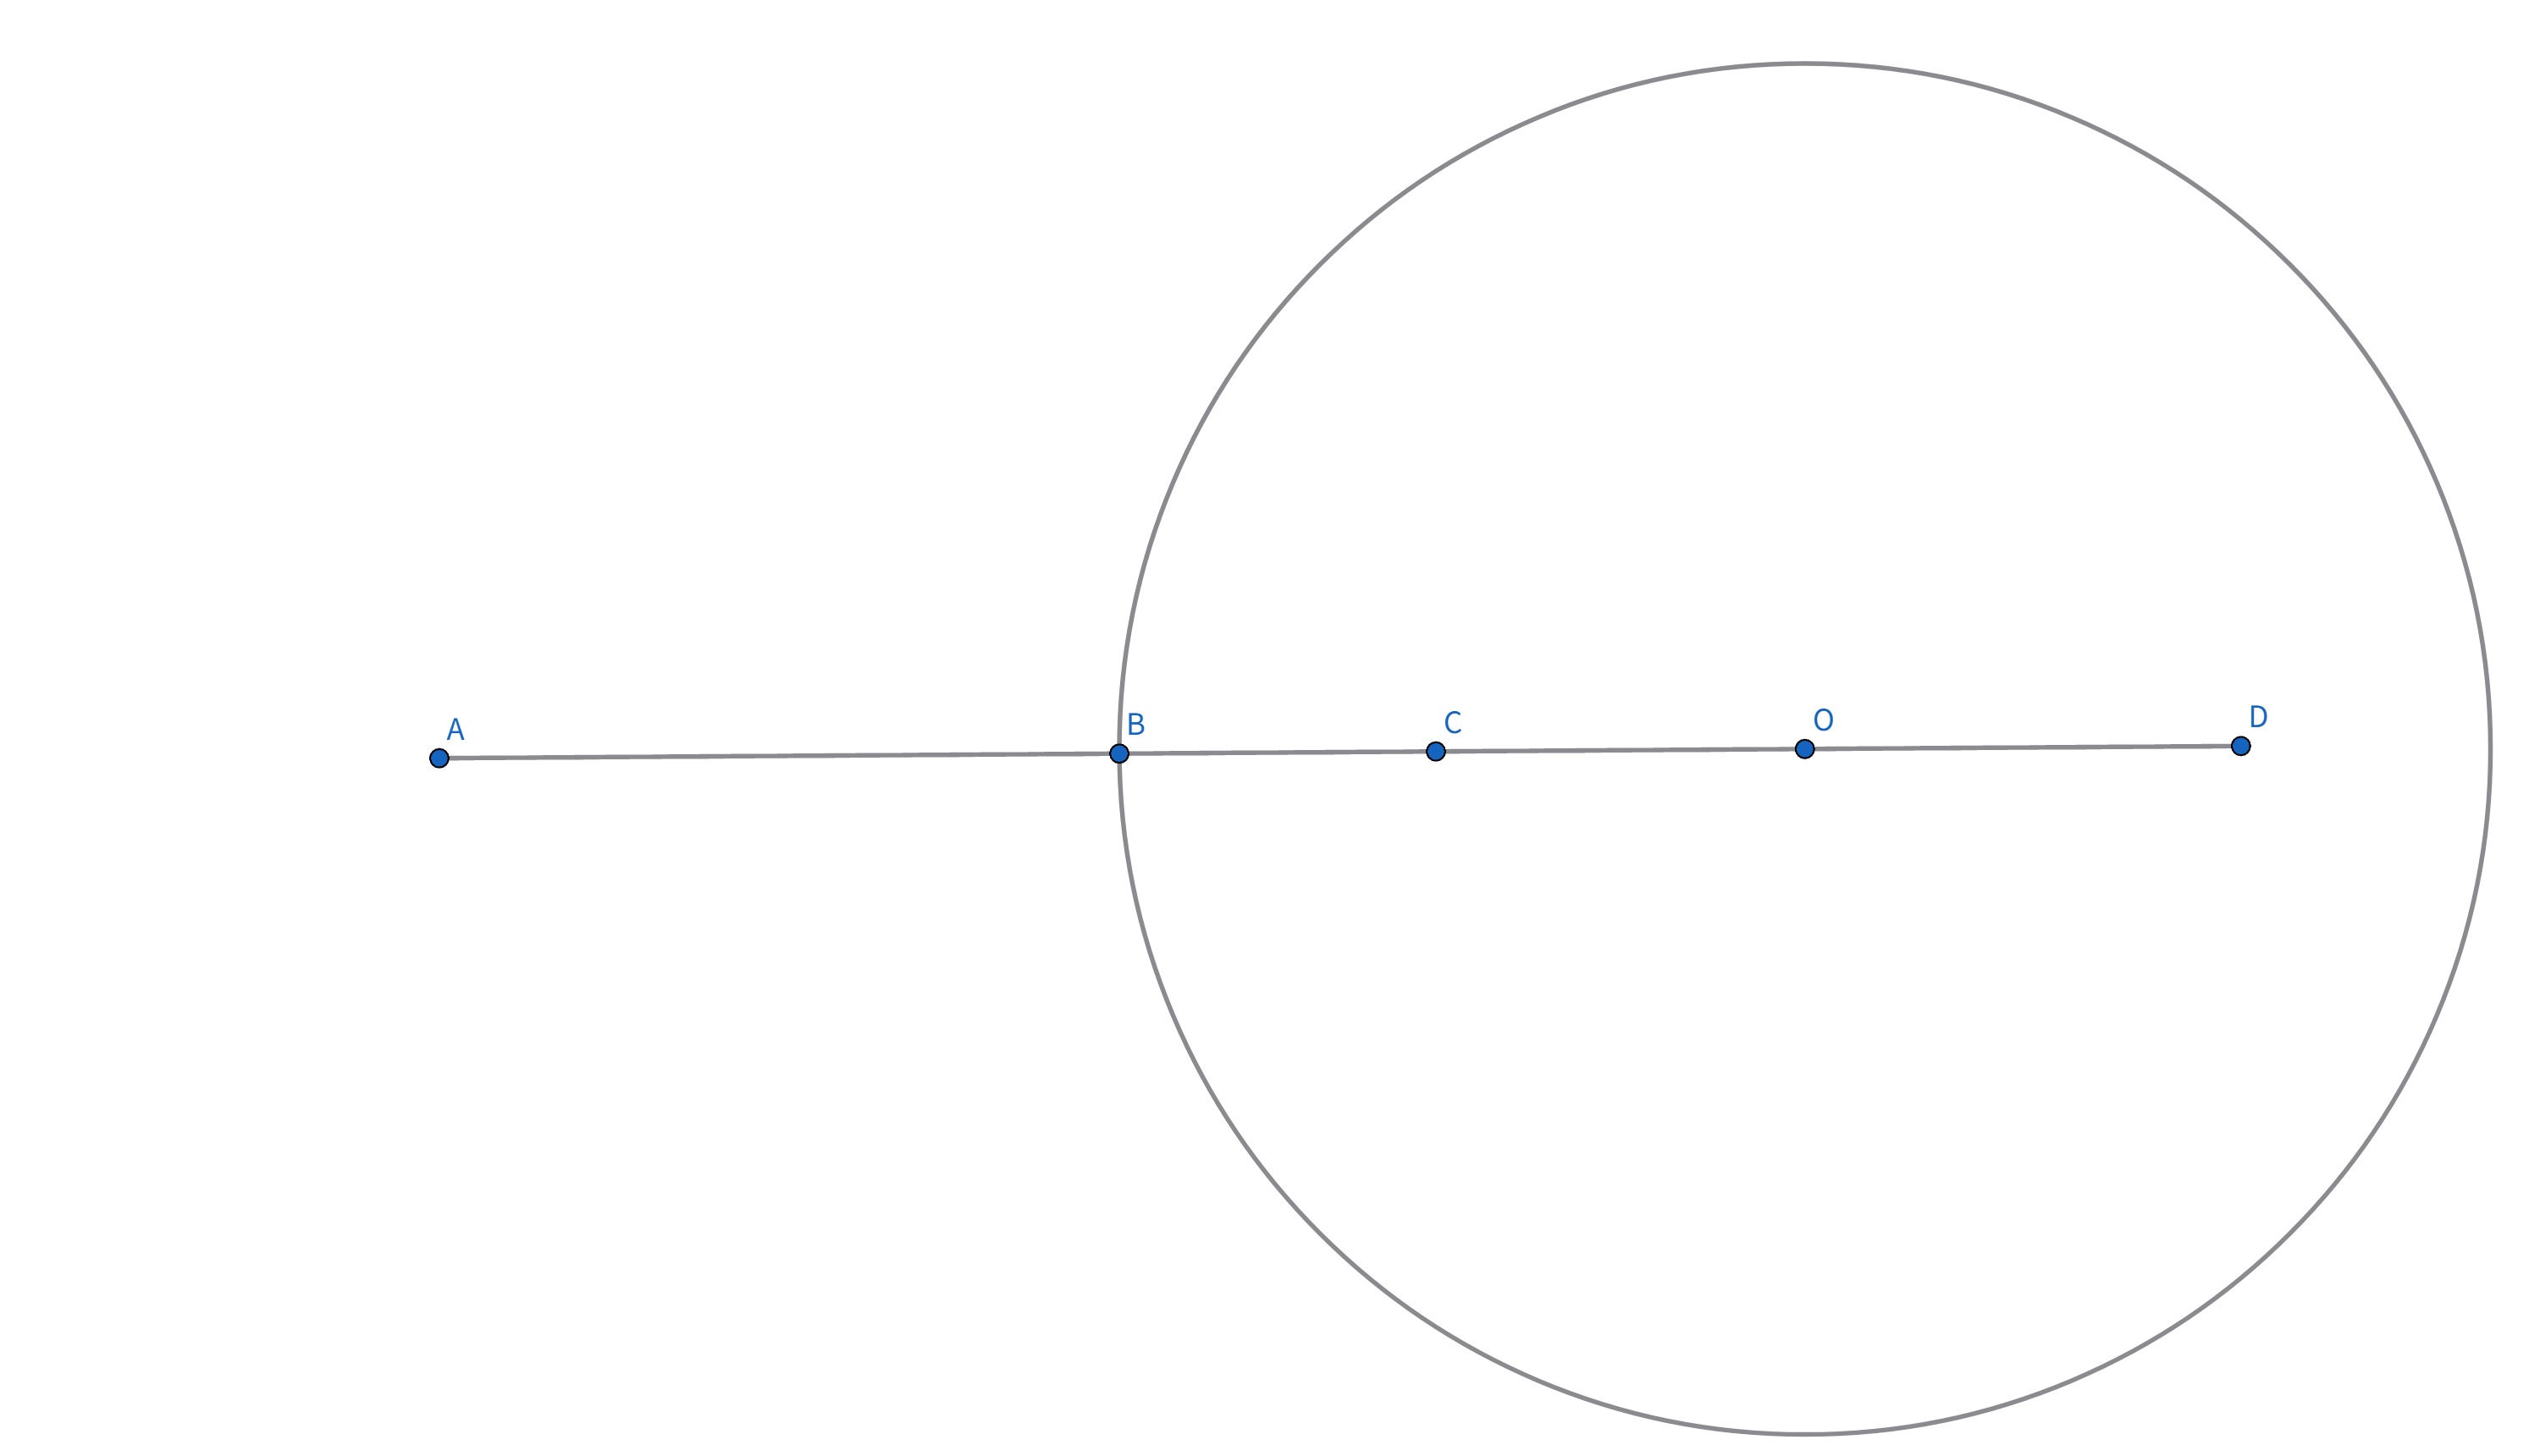
\includegraphics[width=0.8\linewidth]{figures/点与圆.png}
    % \caption{Caption}
    % \label{fig:enter-label}
\end{figure}

设XY为圆O的直径,$\angle XPY$也可以反应点P与圆O的关系。
\begin{itemize}
    \item 点在圆外:$\angle XAY< 90^\circ$。
    \item 点在圆上:$\angle XBY= 90^\circ$。
    \item 点在圆内:$\angle XCY > 90^\circ$。
\end{itemize}
\begin{figure}[H]
    \centering
    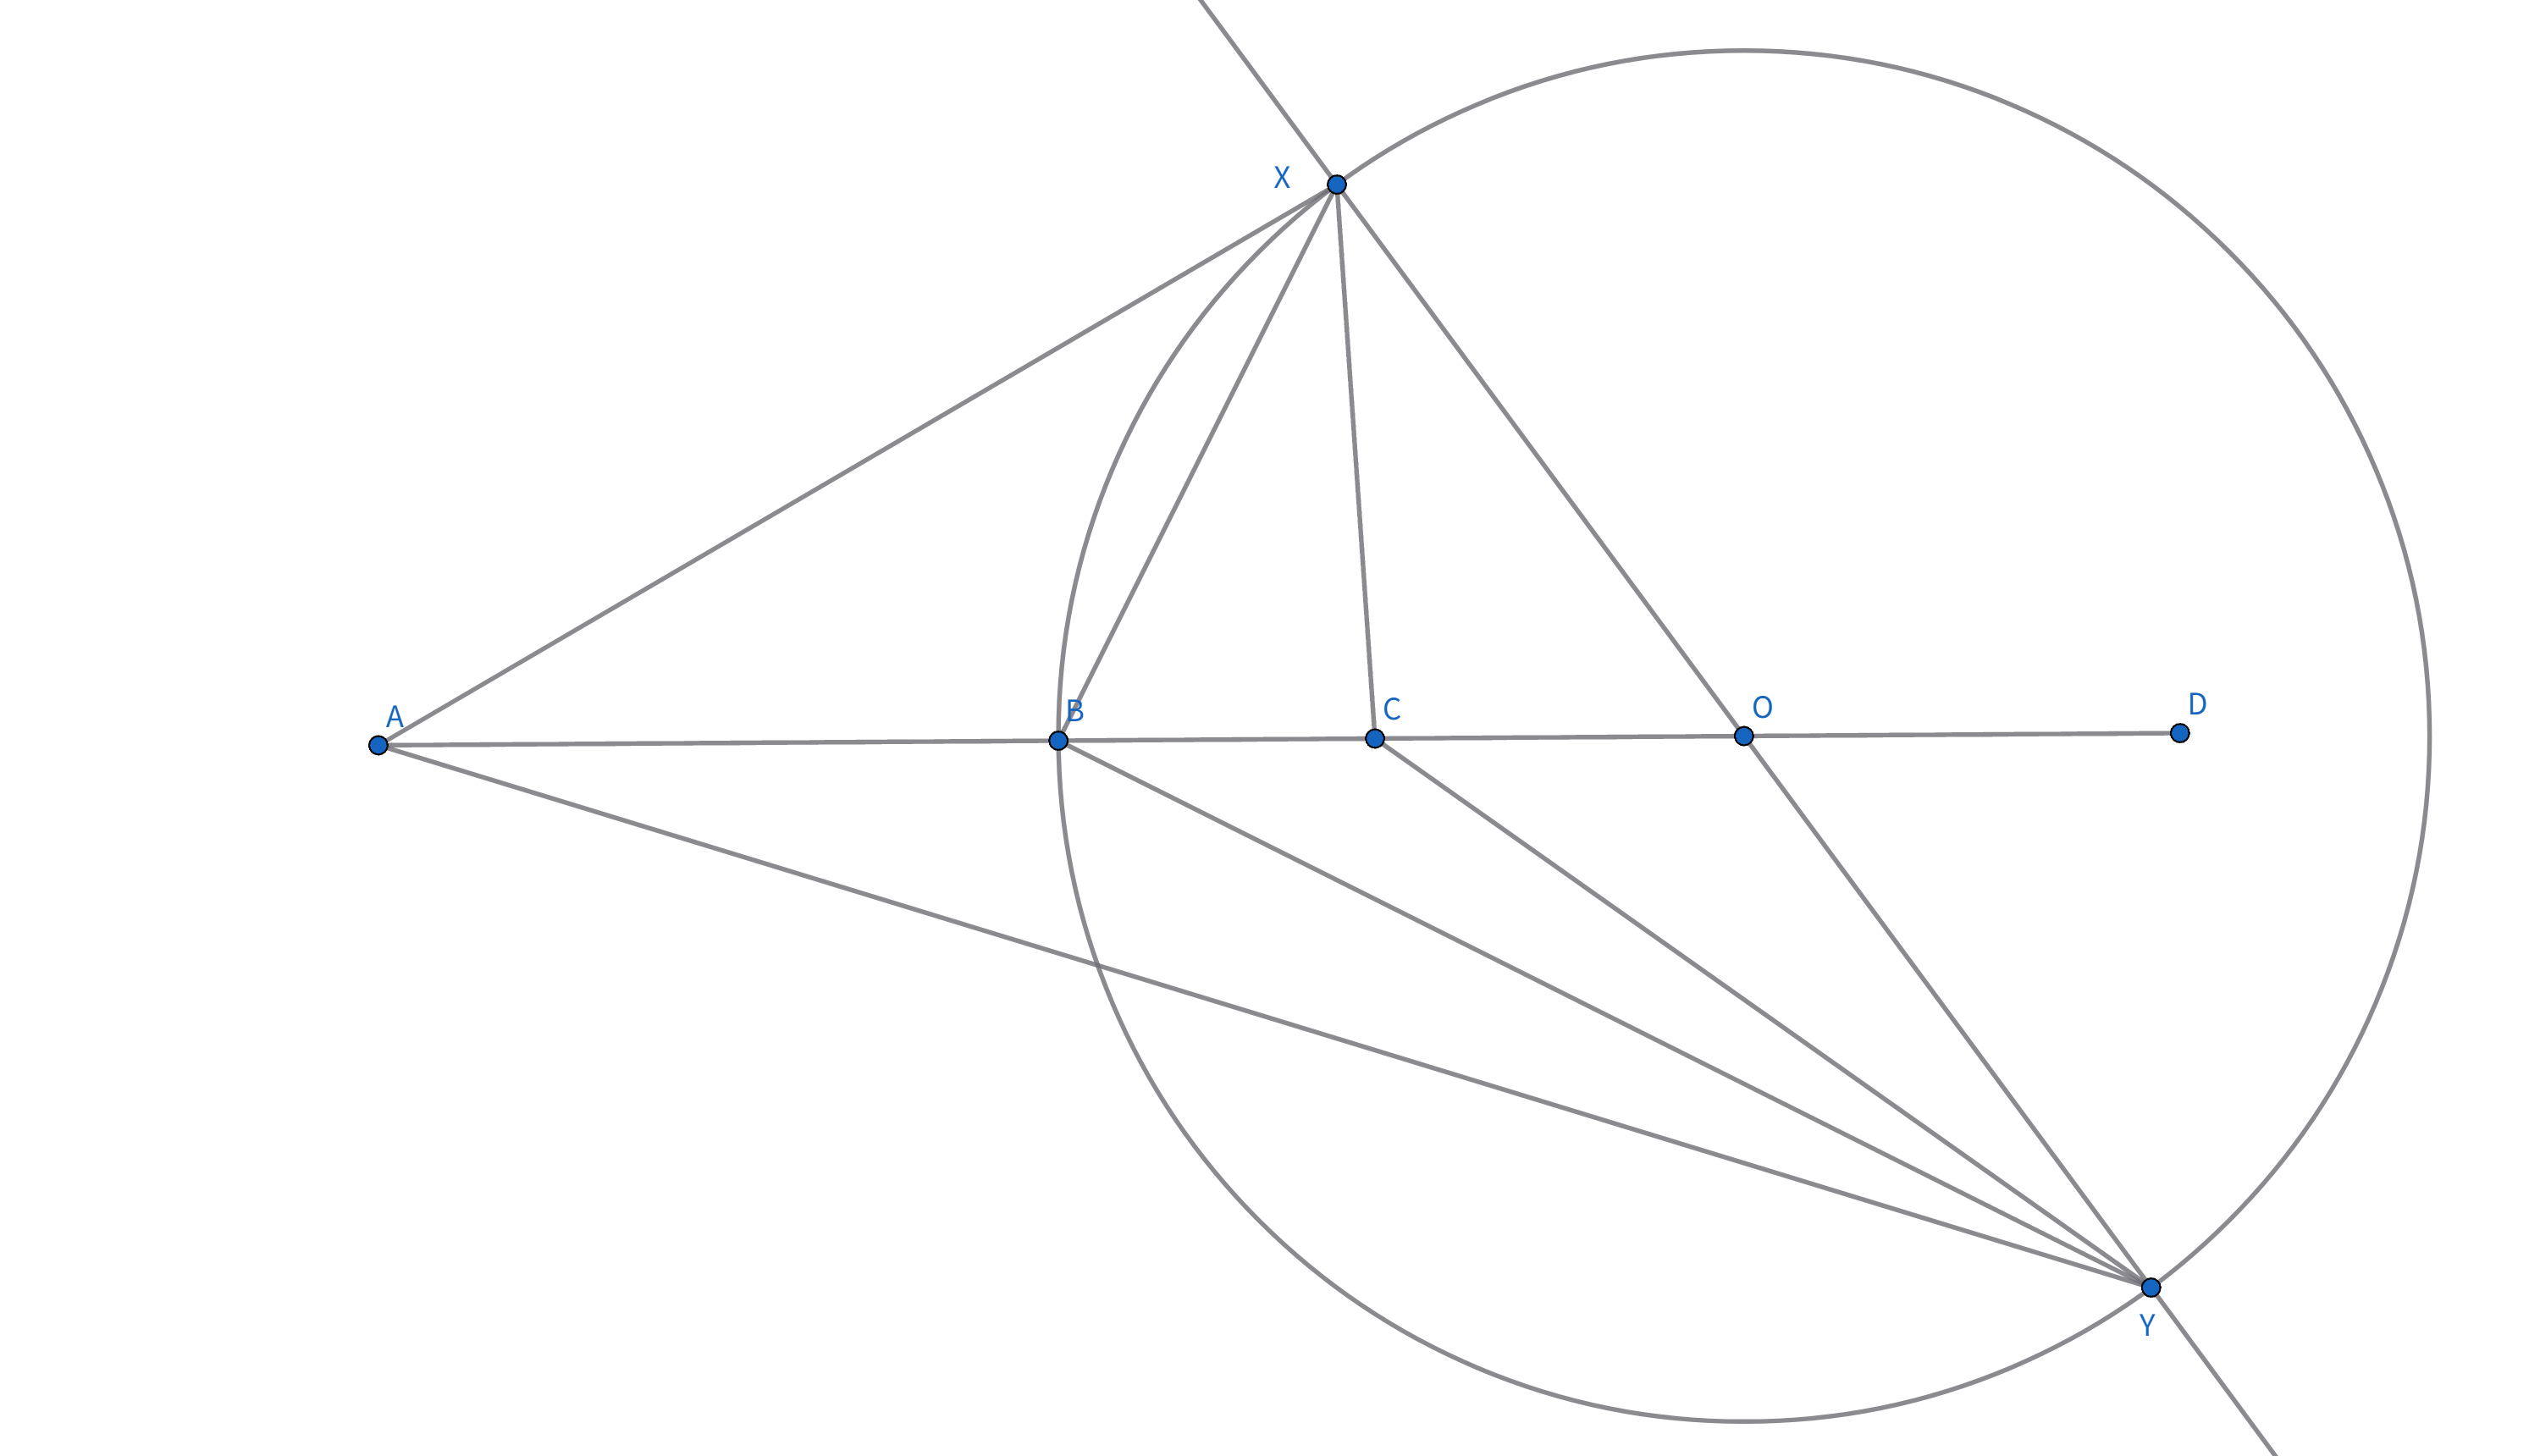
\includegraphics[width=0.8\linewidth]{figures/点与圆2.png}
    % \caption{Caption}
    % \label{fig:enter-label}
\end{figure}

\begin{example}
    对任意凸四边形ABCD以及形内一点P,以四边为直径作圆,则P至少在一个圆的内部。
\end{example}



\section{直线与圆的位置关系}
考虑直线l与圆O的交点个数,或圆心到直线的距离,可以将直线与圆的位置关系分为三类。
\begin{itemize}
    \item 相离:$d(O,l_1)=OA > r$, 直线与圆无交点。
    \item 相切:$d(O,l_1)=OA > r$, 直线与圆恰好有一个交点。称直线$l$ 为圆O的切线,交点称作切点。
    \item 相交:$d(O,l_1)=OA > r$, 直线与圆有两个交点。称$l$ 为圆O的割线,交点AB的连线段为圆O的弦。
\end{itemize}
\begin{figure}[H]
    \centering
    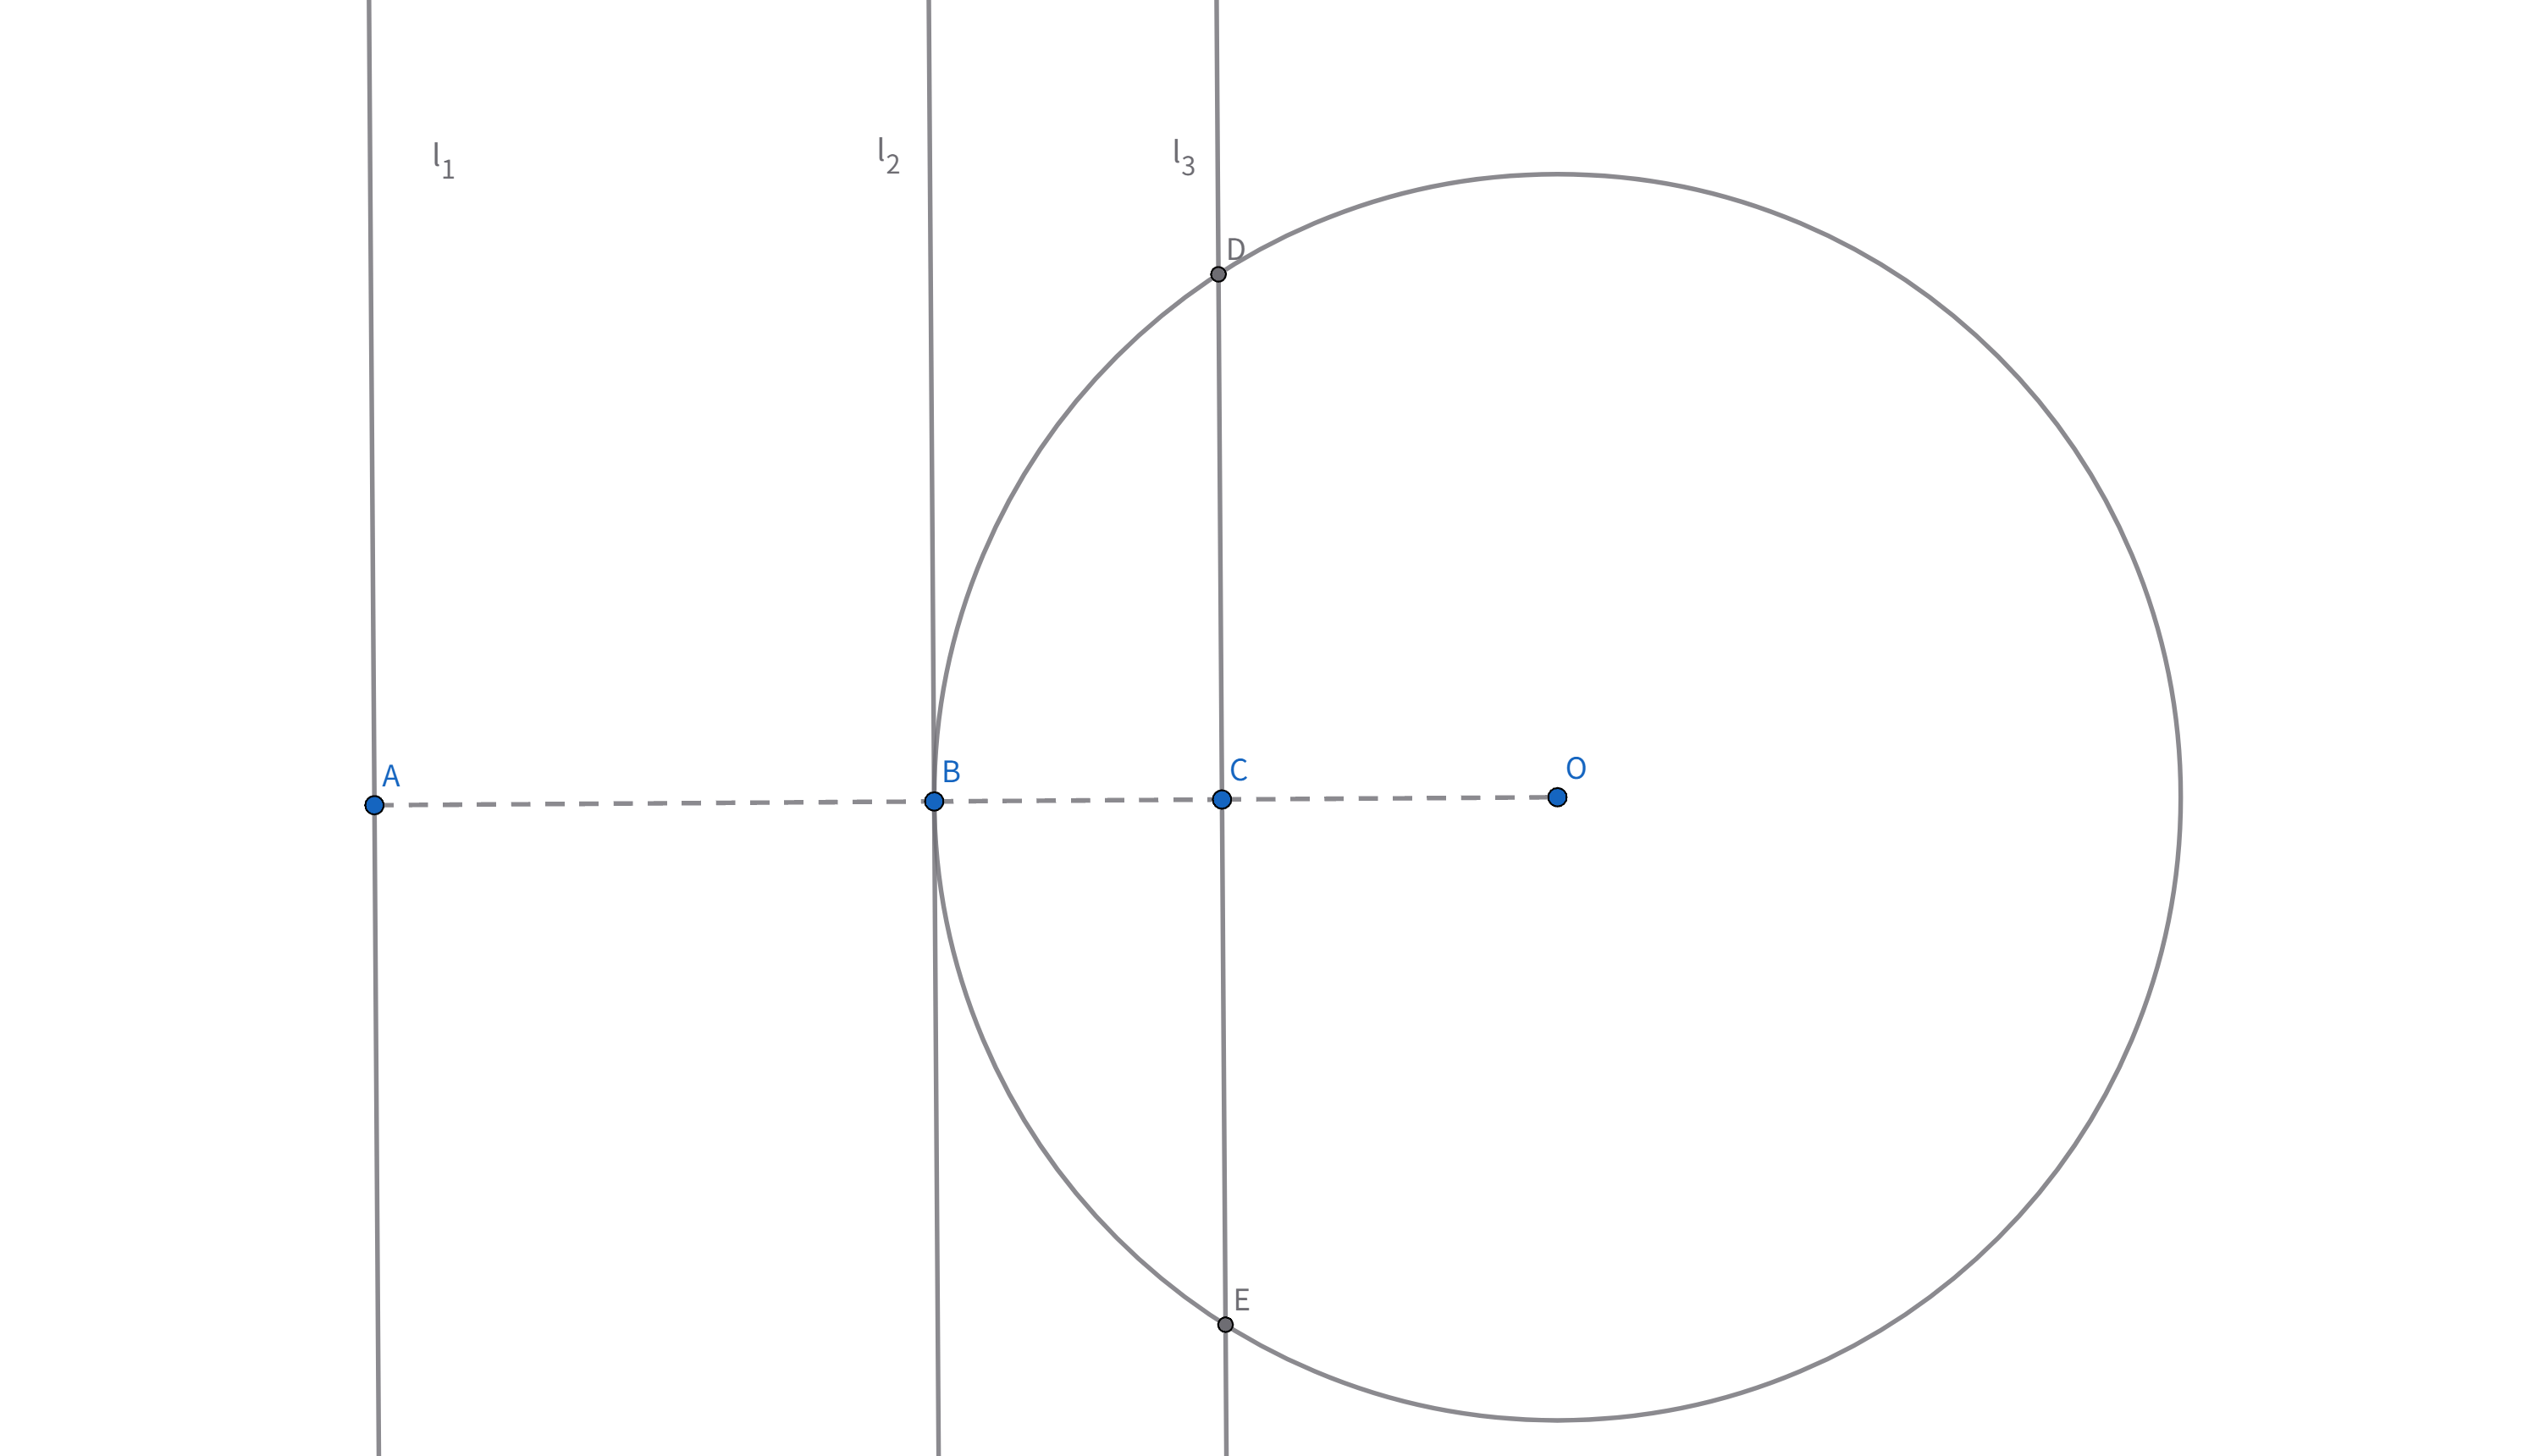
\includegraphics[width=0.8\linewidth]{figures/直线与圆.png}
    % \caption{Caption}
    % \label{fig:enter-label}
\end{figure}



\subsection{切线}
过圆外一点可作2条圆的切线,过圆上一点可做1条圆的切线。
\begin{figure}[H]
    \centering
    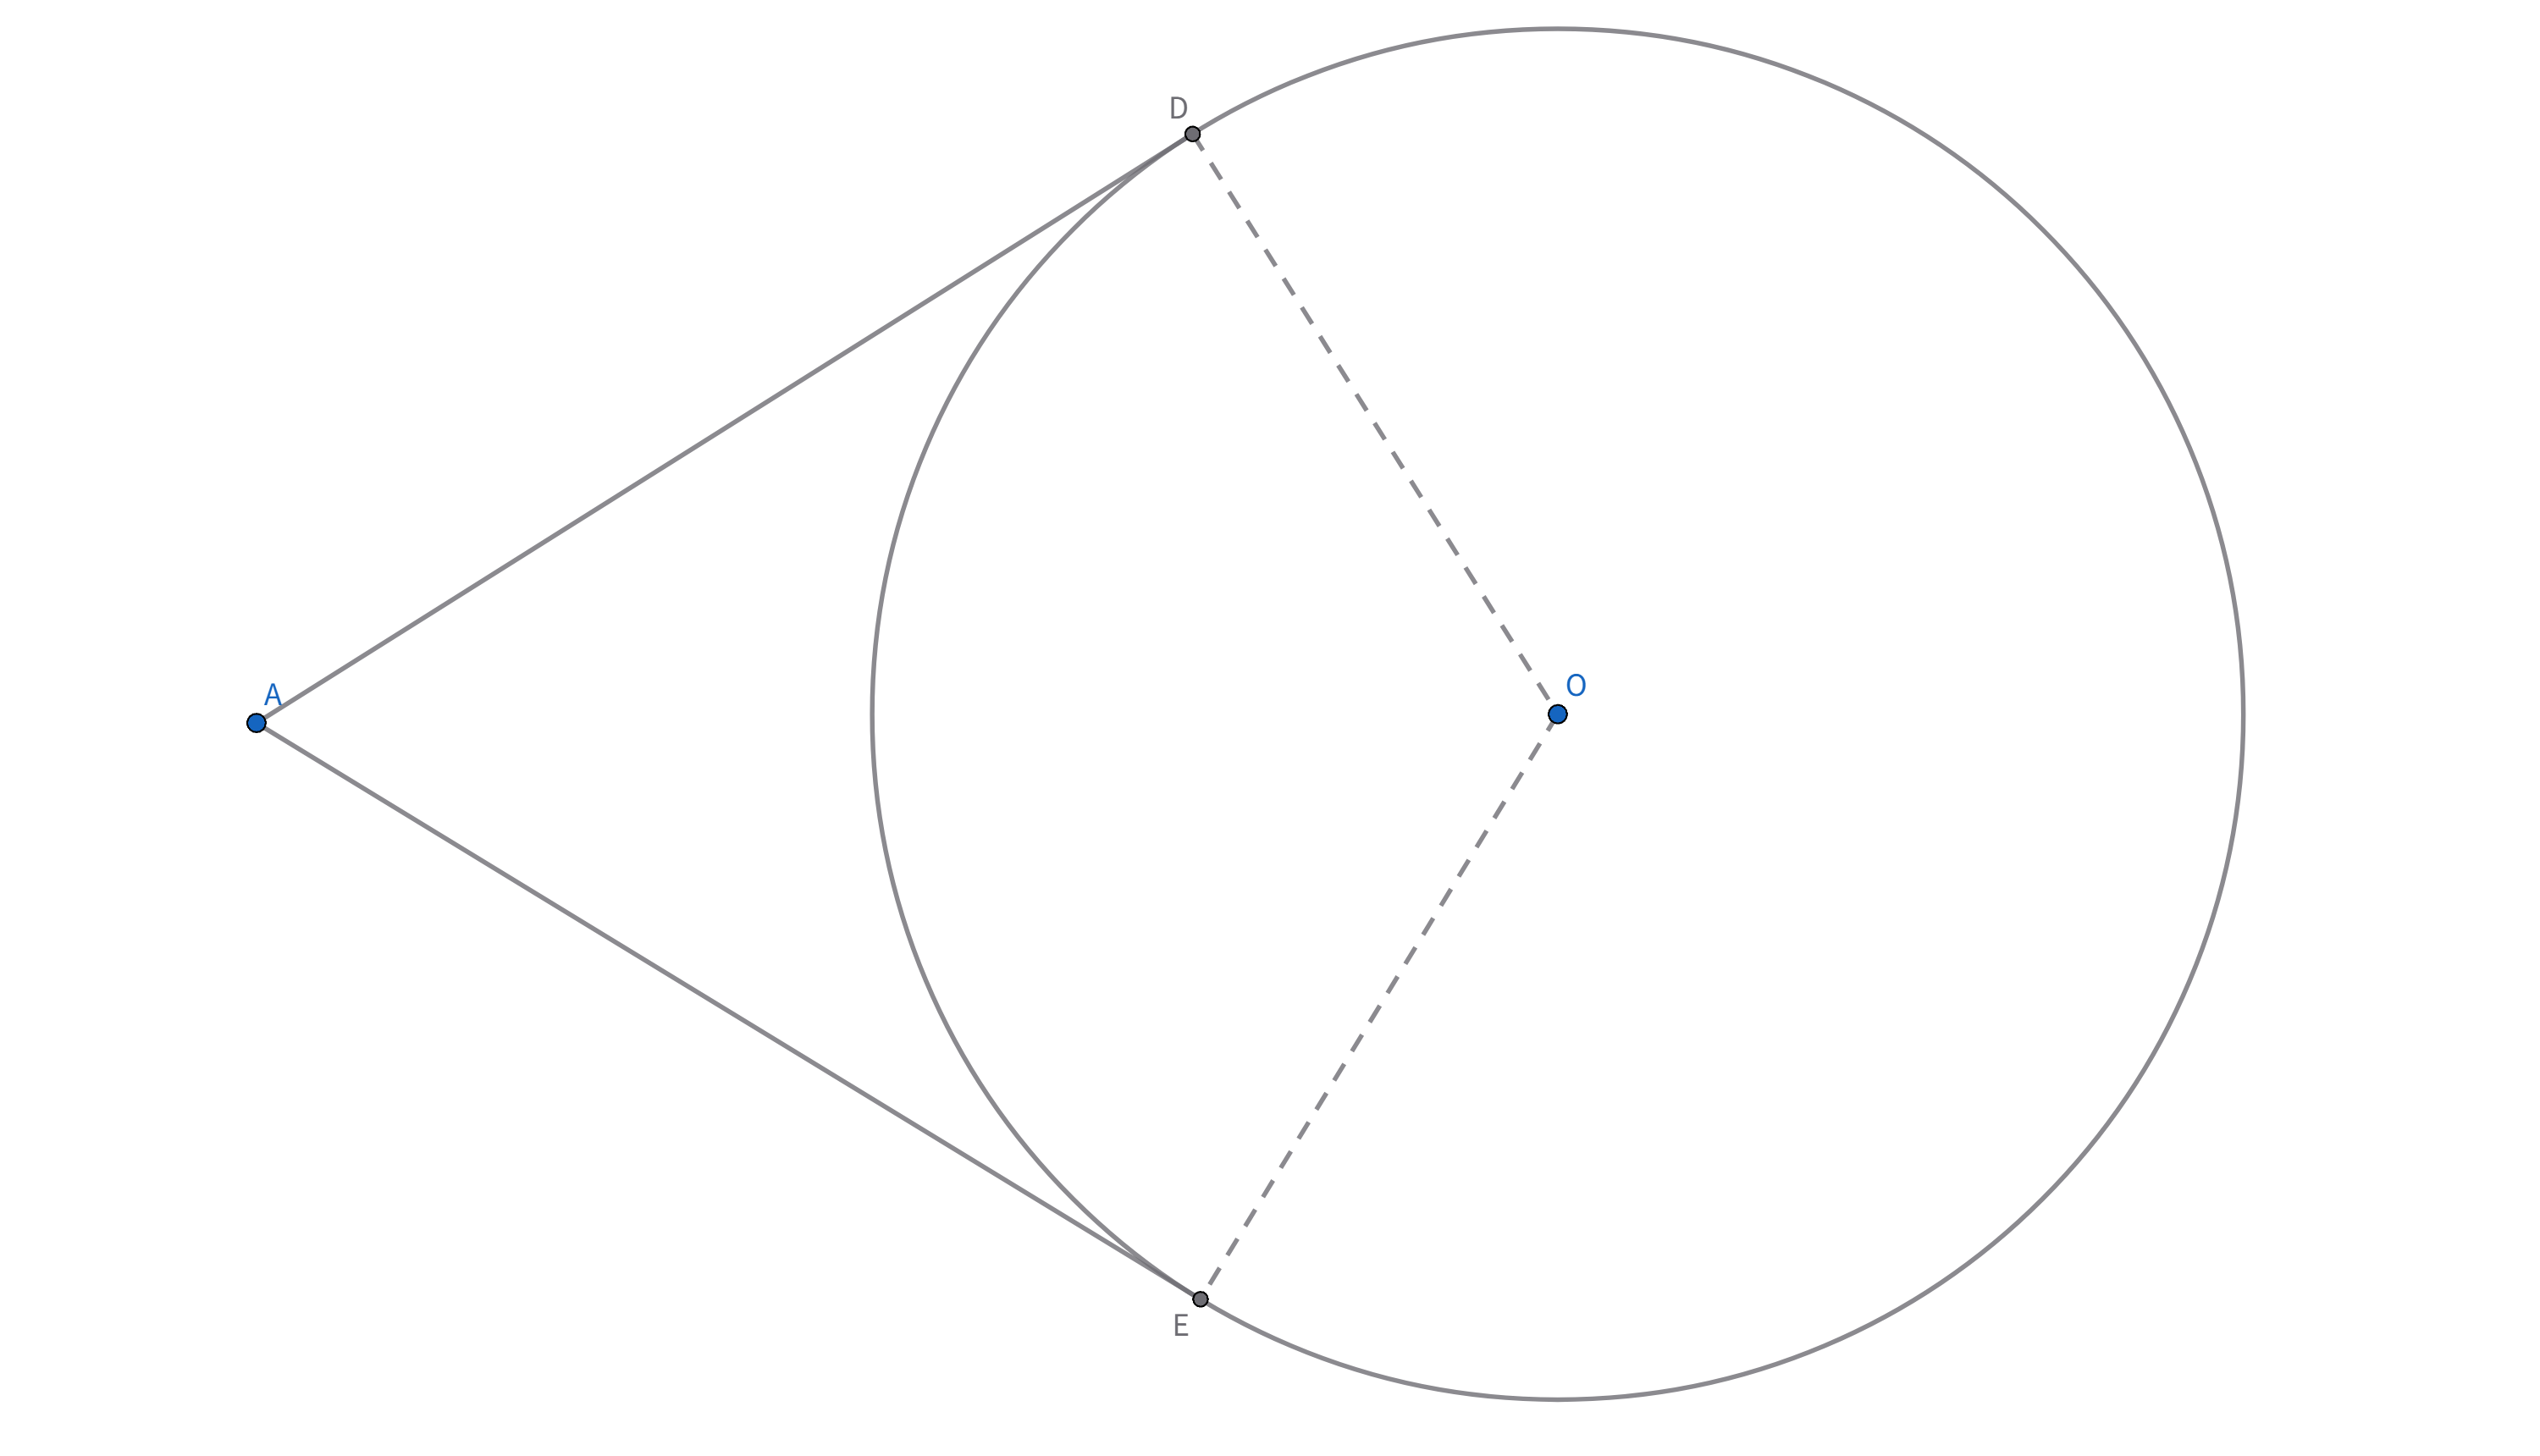
\includegraphics[width=0.8\linewidth]{figures/切线.png}
    % \caption{Caption}
    % \label{fig:enter-label}
\end{figure}
若过圆外一点A作圆O的两条切线,切点为D、E,那么一定有$\angle ADO=\angle AEO$。

过圆心O做直线l的垂线,点O到直线的距离$d(O,l)$可以反应点P与圆O的关系。
\begin{itemize}
    \item 相离:。
    \item 相切:$d(O,l_2) = OB = r$。
    \item 相交:$d(O,l_3) = OC < r$。
\end{itemize}
连接圆心O与切点B,则OB一定垂直于直线$l_2$。




\subsection{相交弦定理}
\begin{theorem}[相交弦定理]
    假设平面内有一半径为R的圆O,E为圆内一定点。过E作任意弦AC、BD,一定有
    $$
    AE \cdot EC =BE \cdot ED = R^2 - EO^2
    $$
\end{theorem}
\begin{figure}[H]
    \centering
    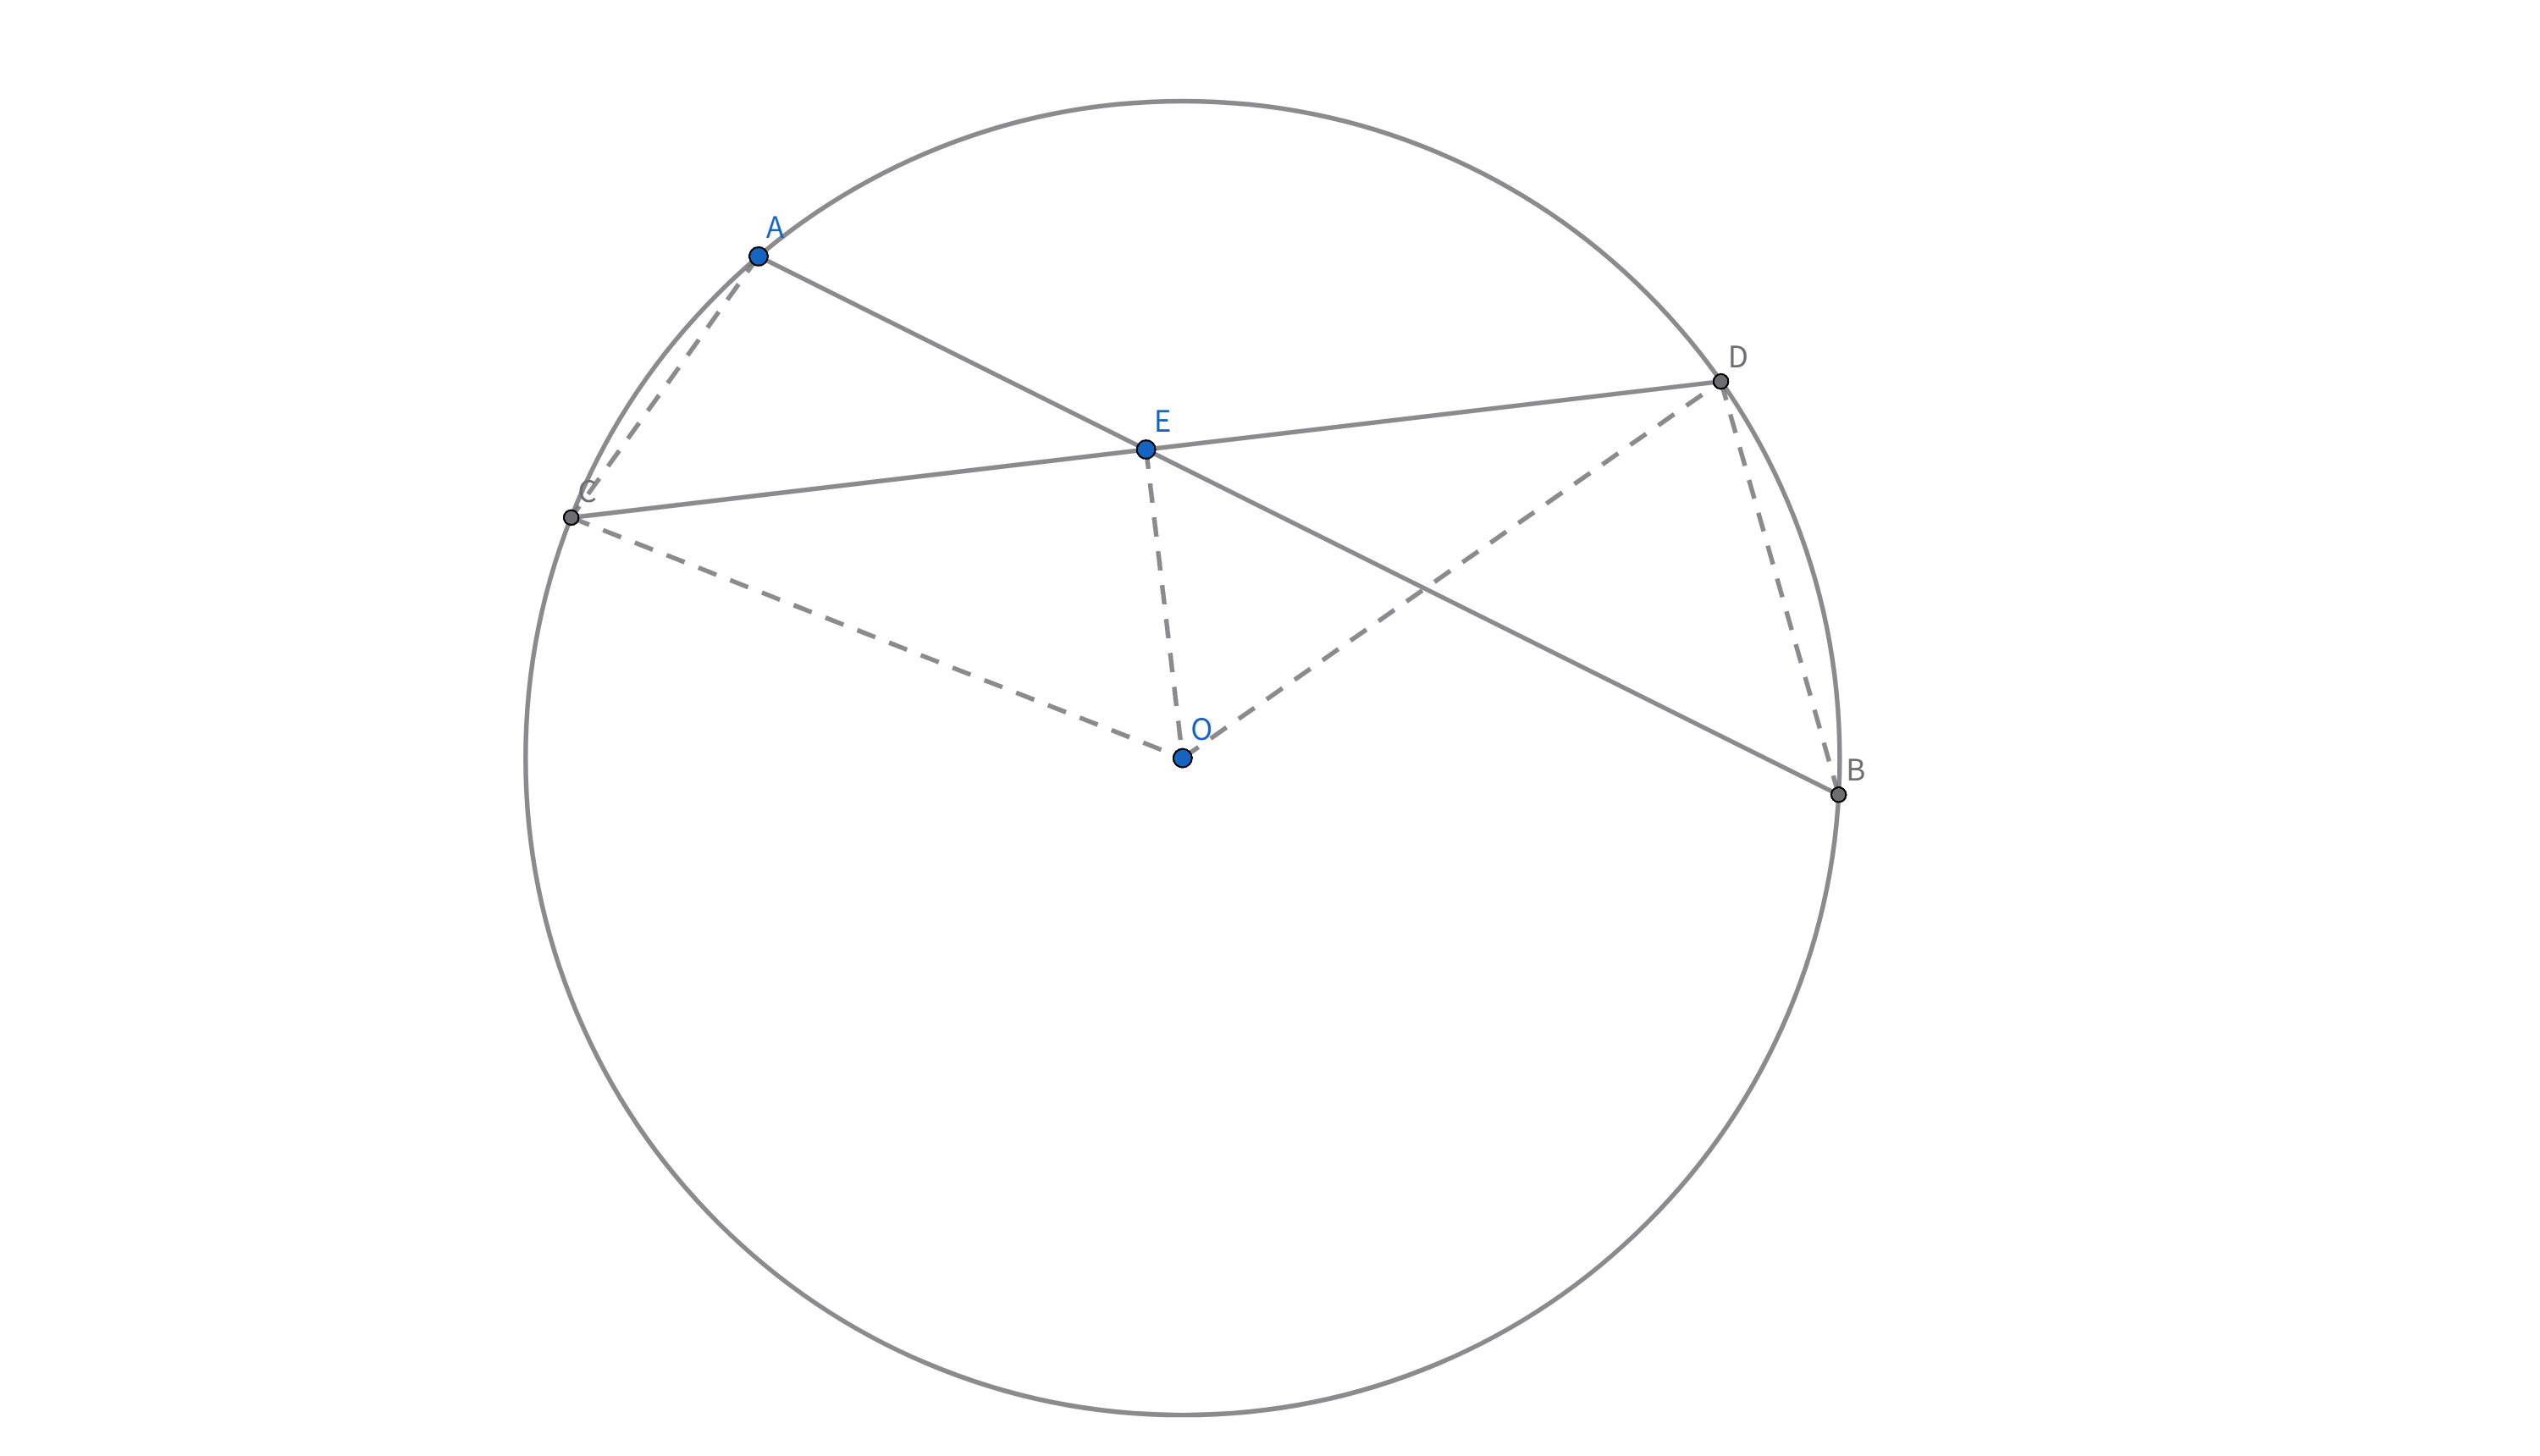
\includegraphics[width=0.7\linewidth]{figures/相交弦定理.png}
    \caption{相交弦定理}
    % \label{fig:enter-label}
\end{figure}


% 割线定理
\subsection{割线定理}
\begin{theorem}[割线定理]
   假设平面内有一半径为R的圆O,E为圆外一定点。过E作两条圆O割线分别交于AB、CD,一定有
$$
EA \cdot EB =EC \cdot ED = EO^2 -R^2
$$
\end{theorem}
\begin{figure}[H]
    \centering
    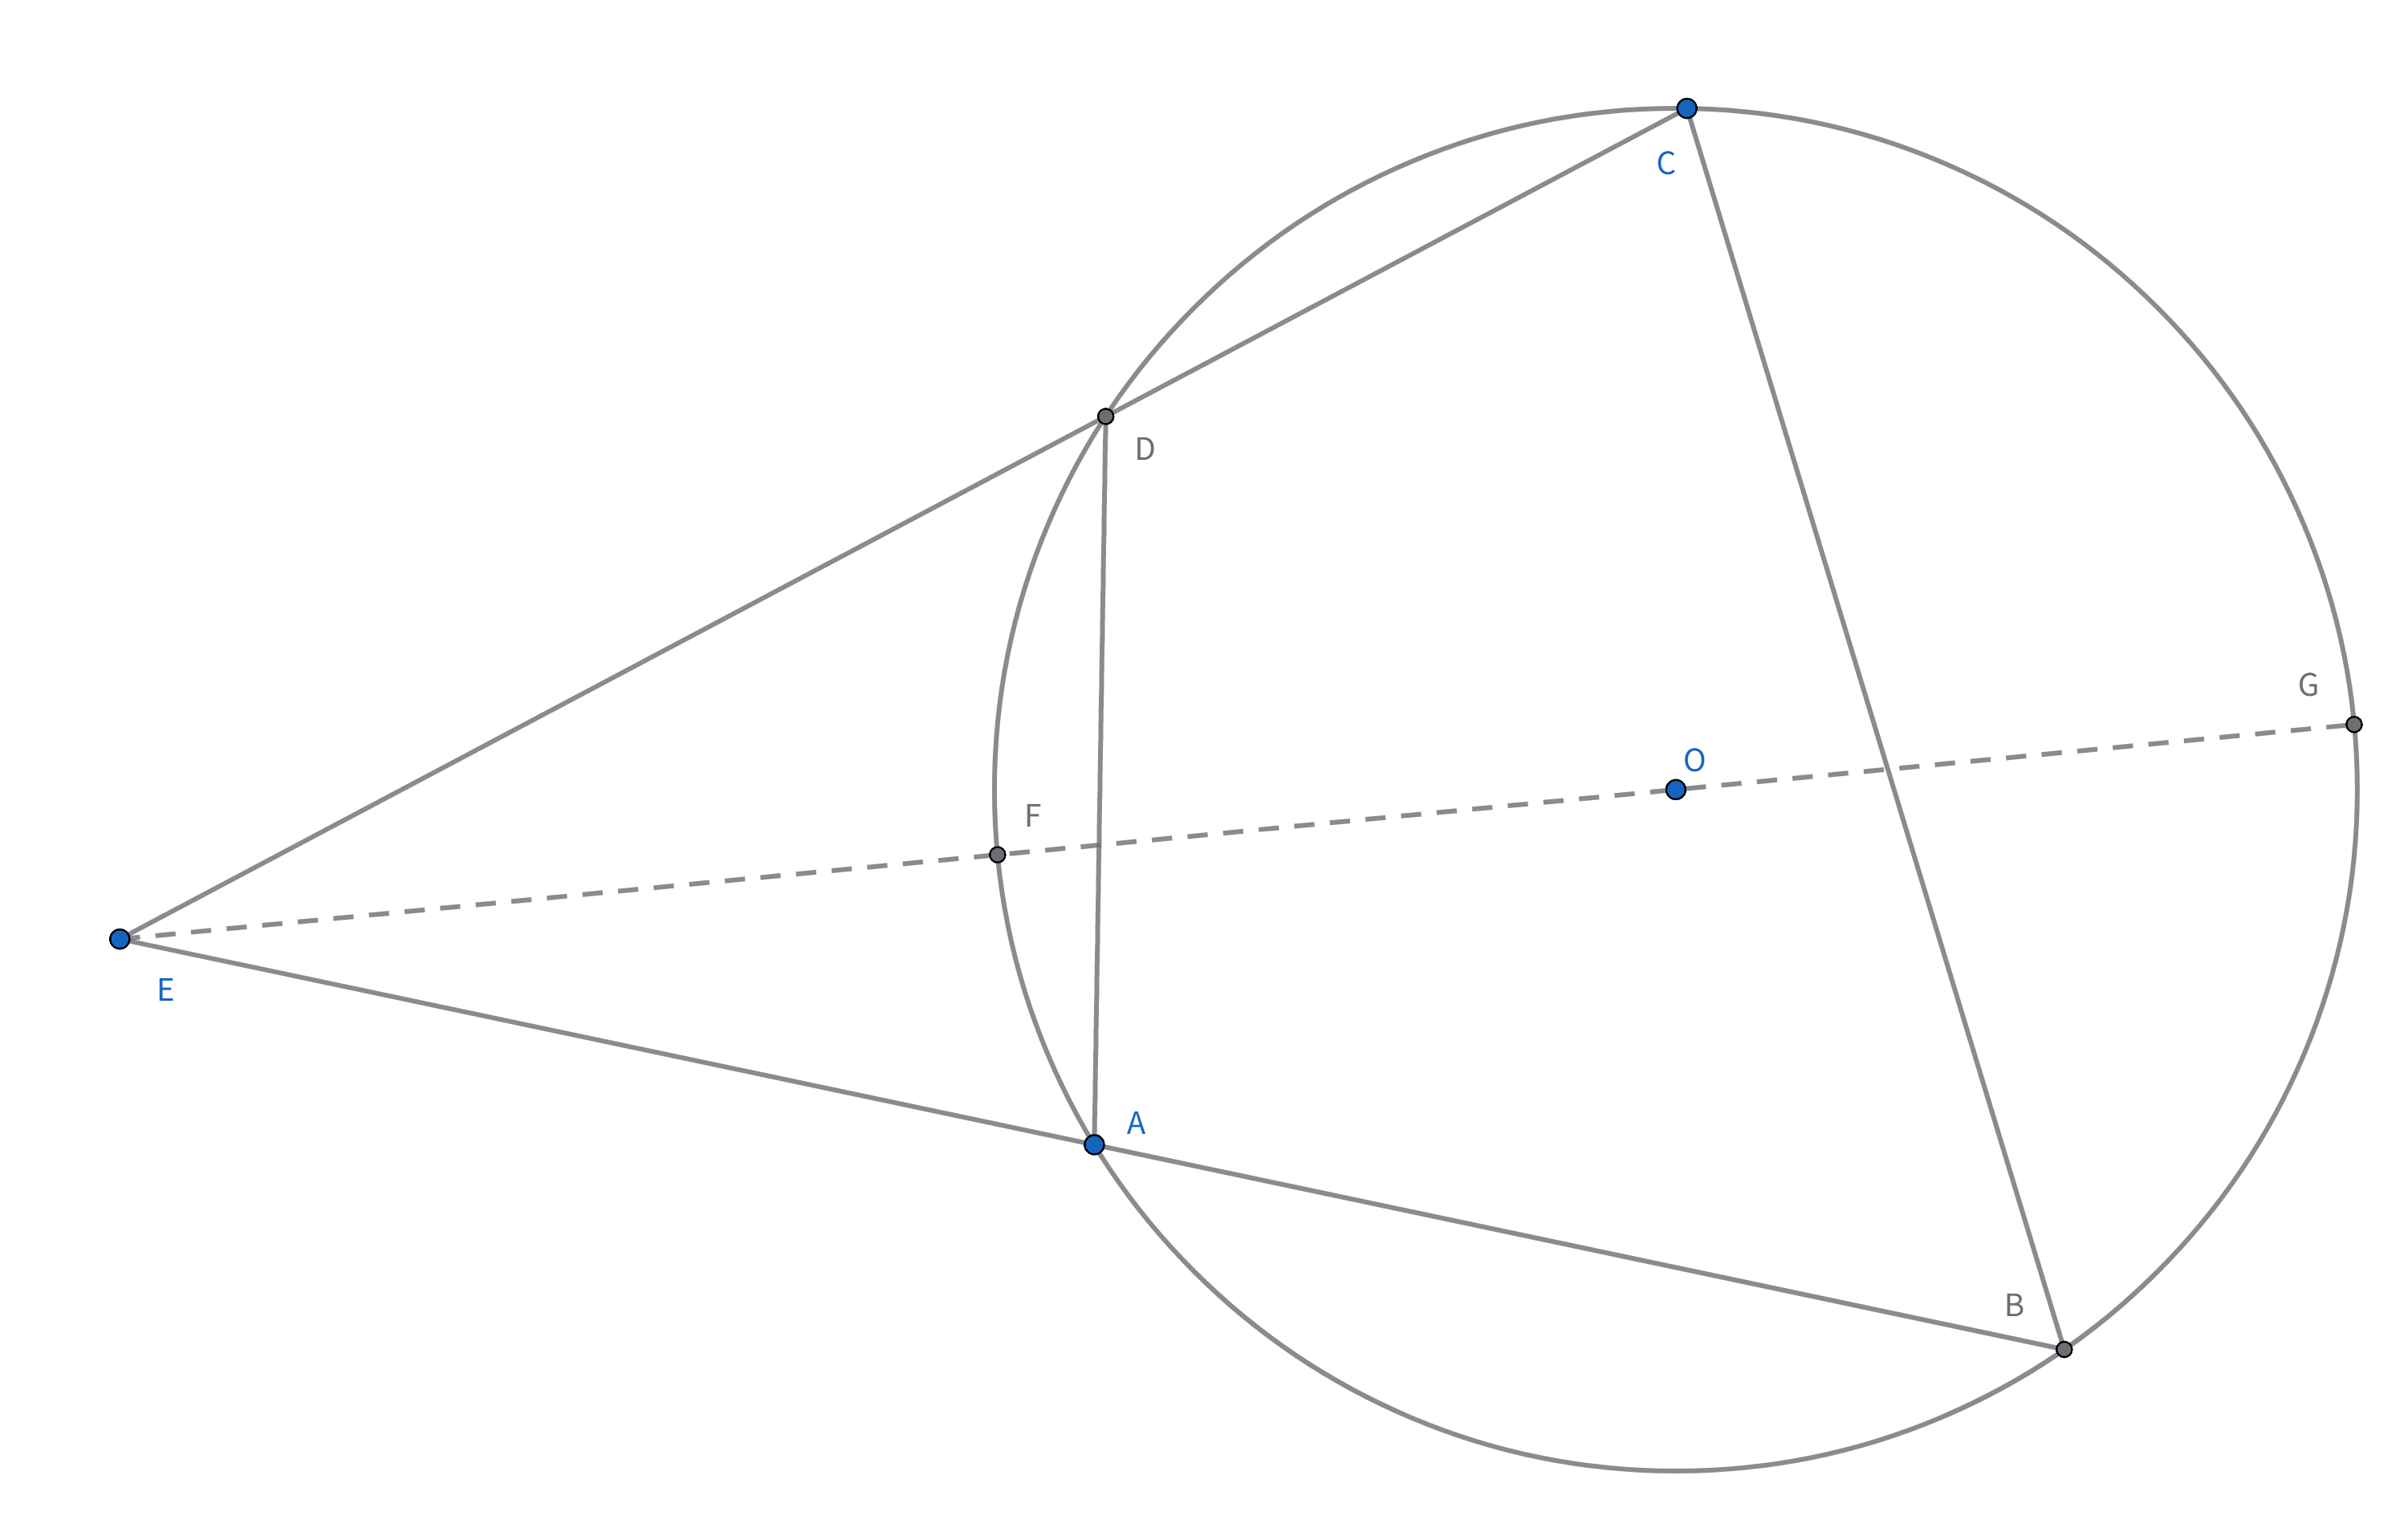
\includegraphics[width=0.7\linewidth]{figures/割线定理.png}
    \caption{割线定理}
    % \label{fig:enter-label}
\end{figure}


% 切割线定理
\section{切割线定理}
\begin{theorem}[切割线定理]
    假设平面内有一半径为R的圆O,E为圆外一定点。过E作任意割线交圆于AC,作切线交圆于B,一定有
    $$
    EB^2 = EA \cdot EC = EO^2 - R^2
    $$
\end{theorem}
\begin{figure}[H]
    \centering
    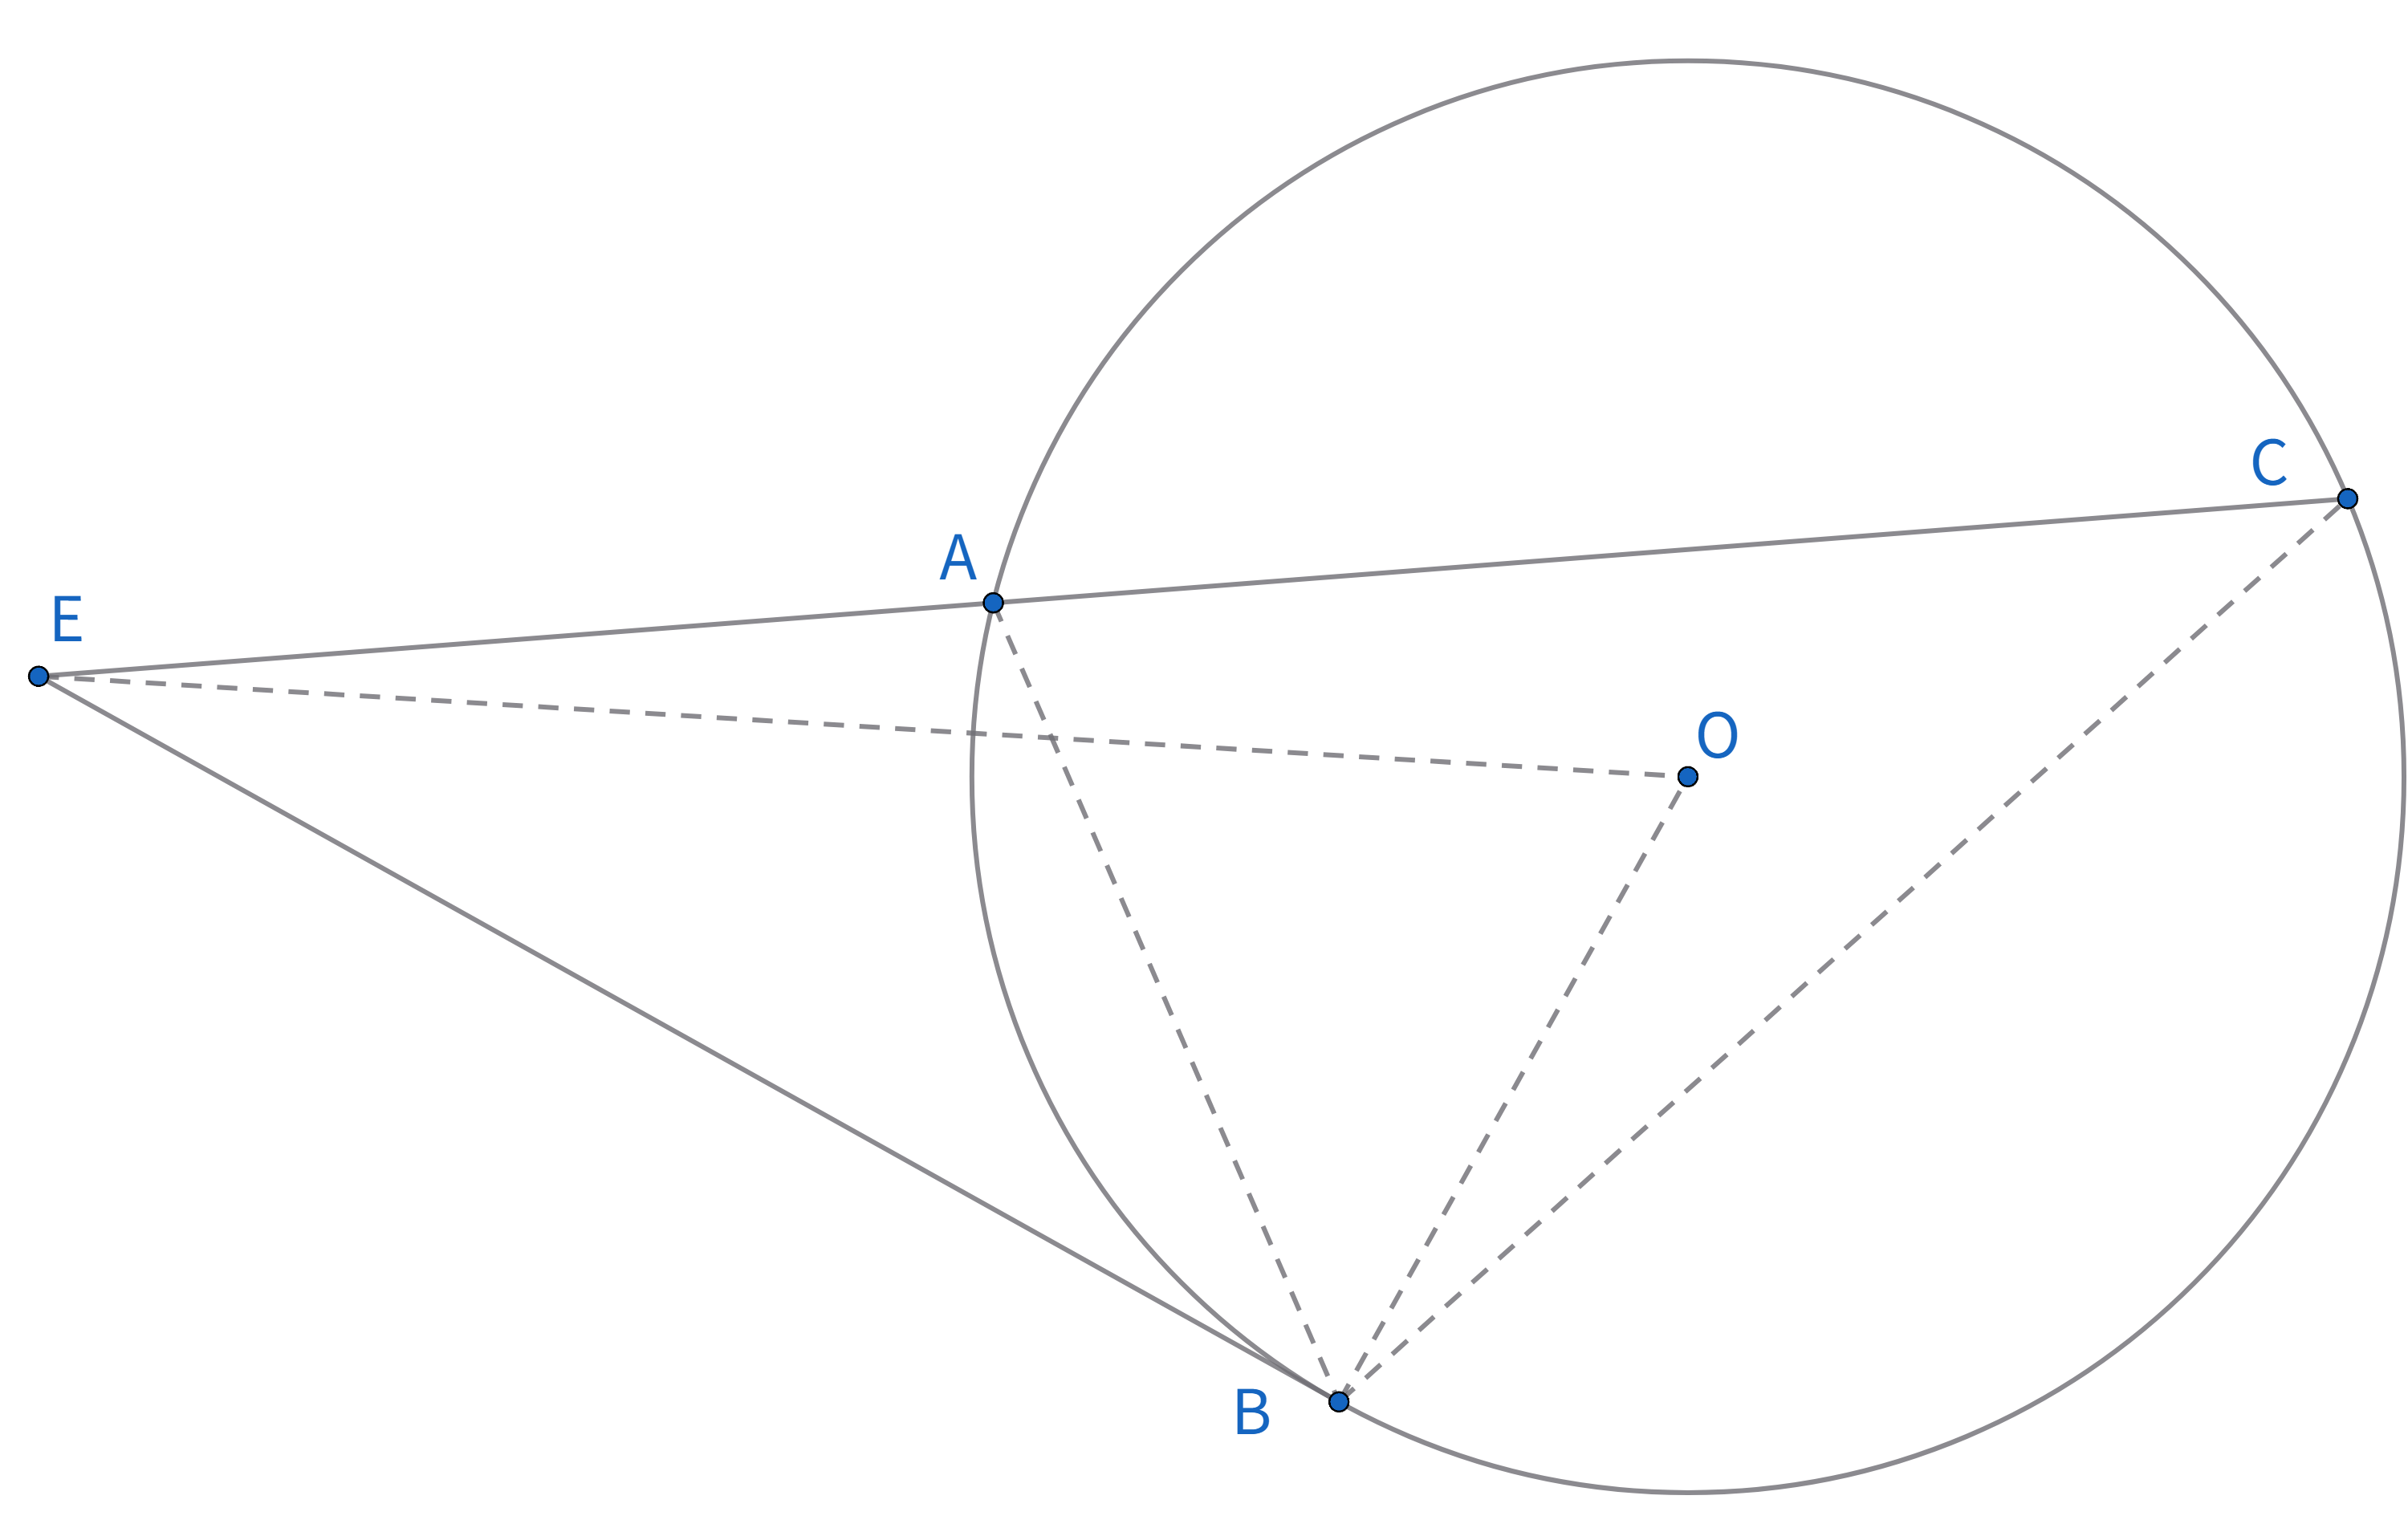
\includegraphics[width=0.7\linewidth]{figures/切割弦定理.png}
    \caption{切割线定理}
\end{figure}


\subsection{圆与圆的位置关系}
圆与圆的位置关系可分为五类,包括外离、外切、相交、内切、内含。
\begin{itemize}
    \item 相离:两圆无交点,可分为外离与内含。
    \item 相切:两圆恰好有一个交点,交点称作切点,可分为外切与内切。
    \item 相交:两圆有两个交点,交点AB构成的连线段称作两圆的相交弦。
\end{itemize}
\begin{figure}[H]
    \centering
    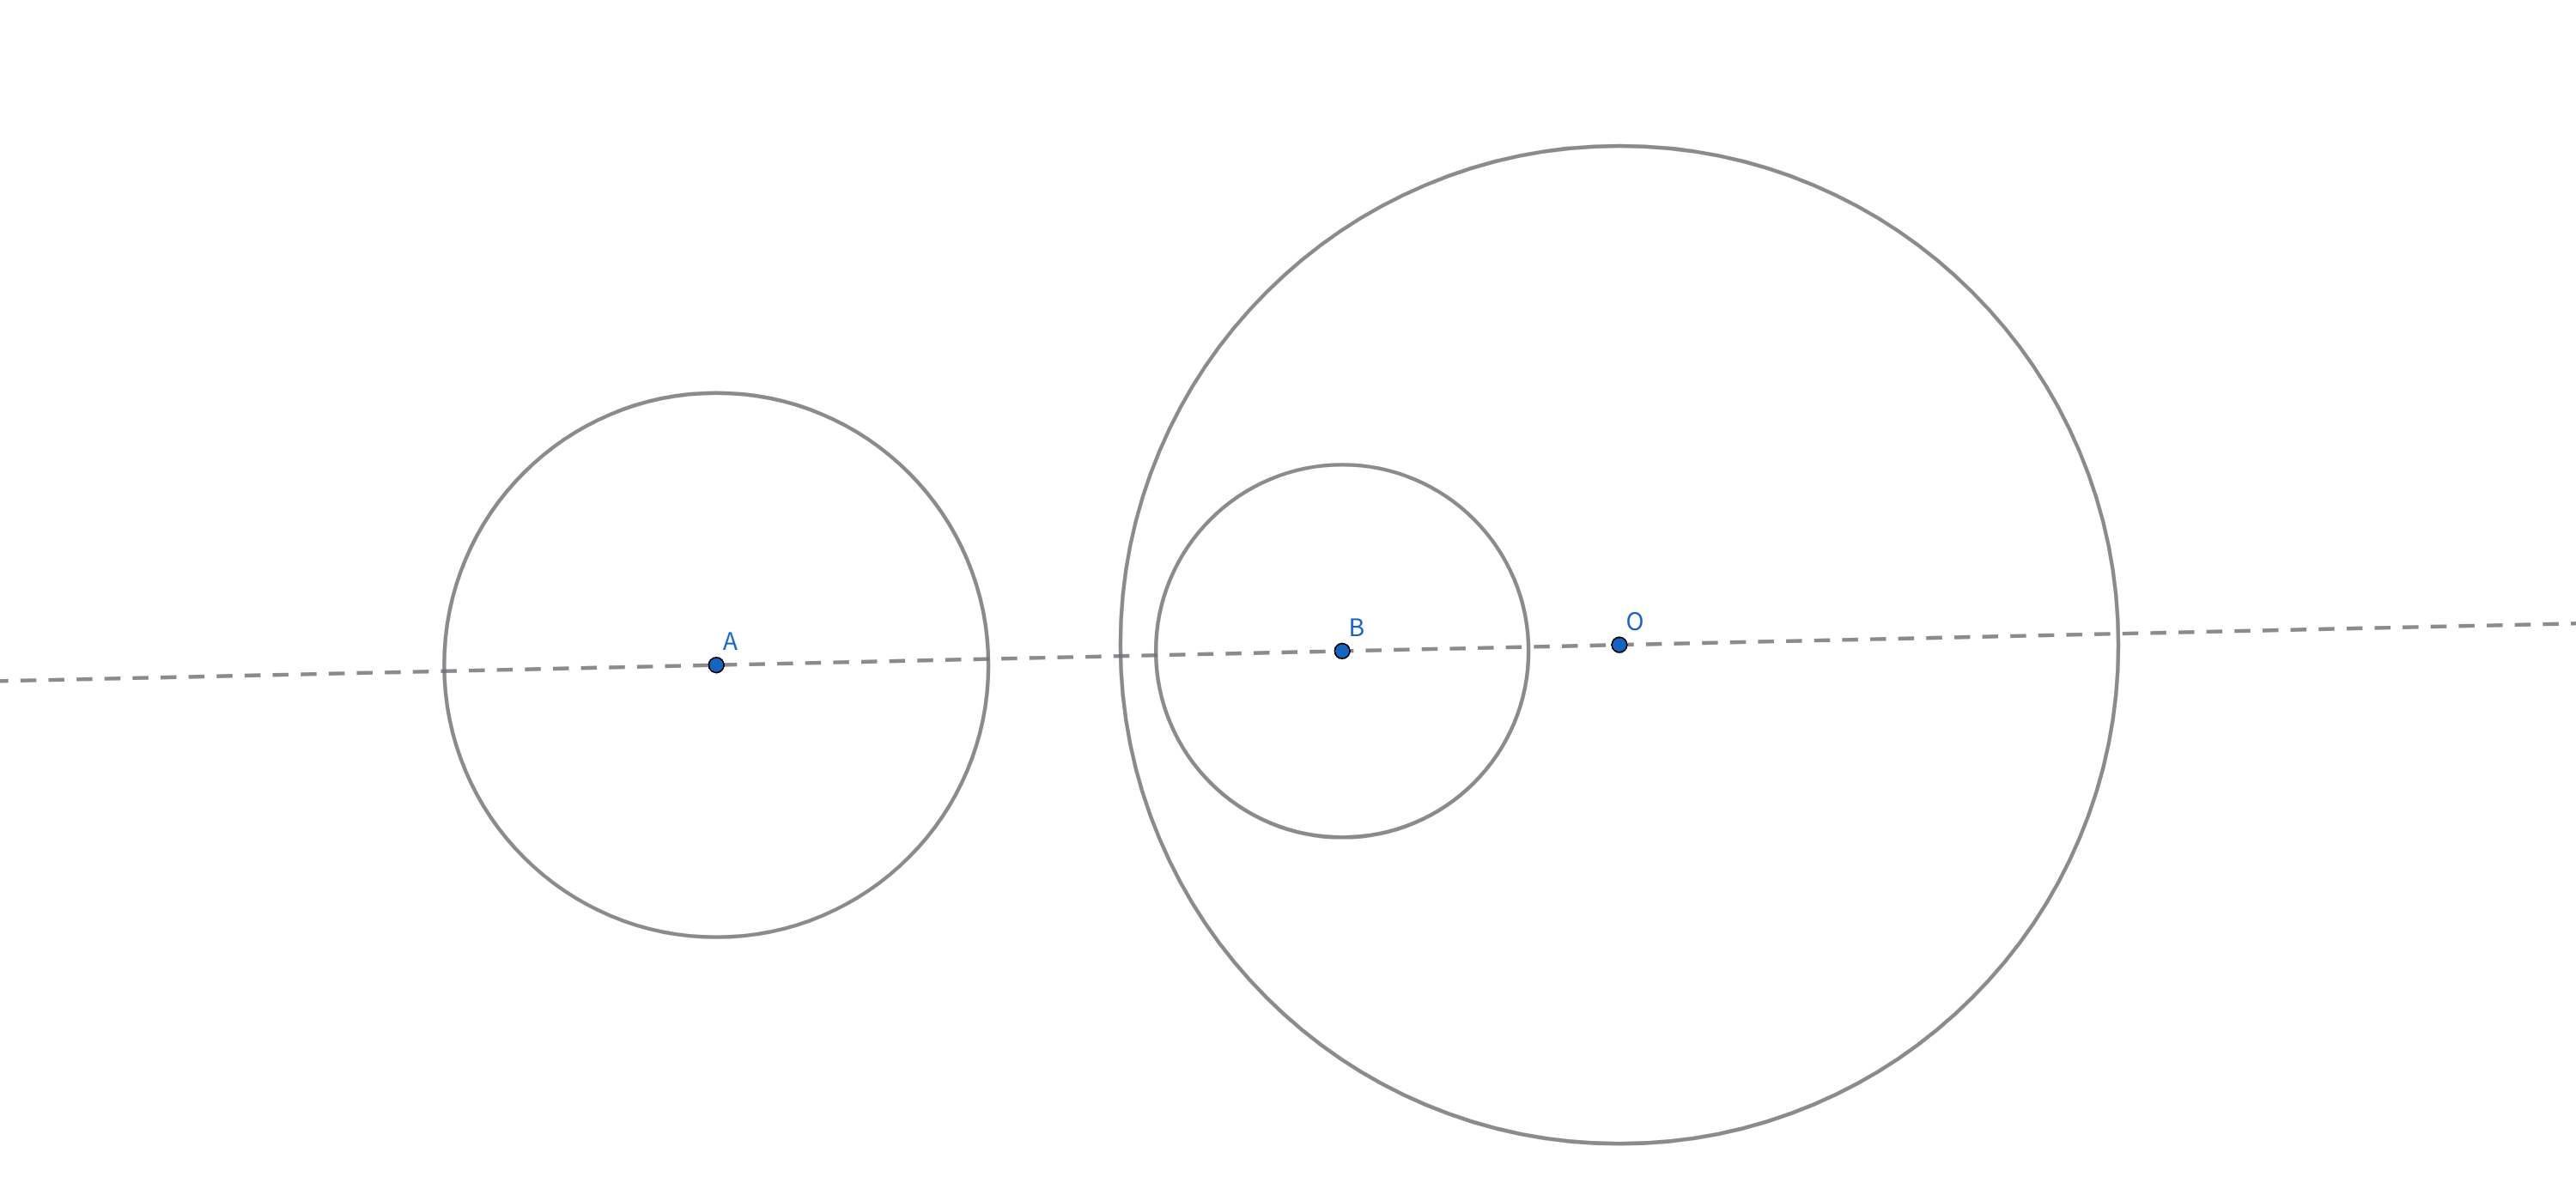
\includegraphics[width=0.5\linewidth]{figures/外离与内含.png}
    \caption{外离与内含}
    % \label{fig:enter-label}
\end{figure}
\begin{figure}[H]
    \centering
    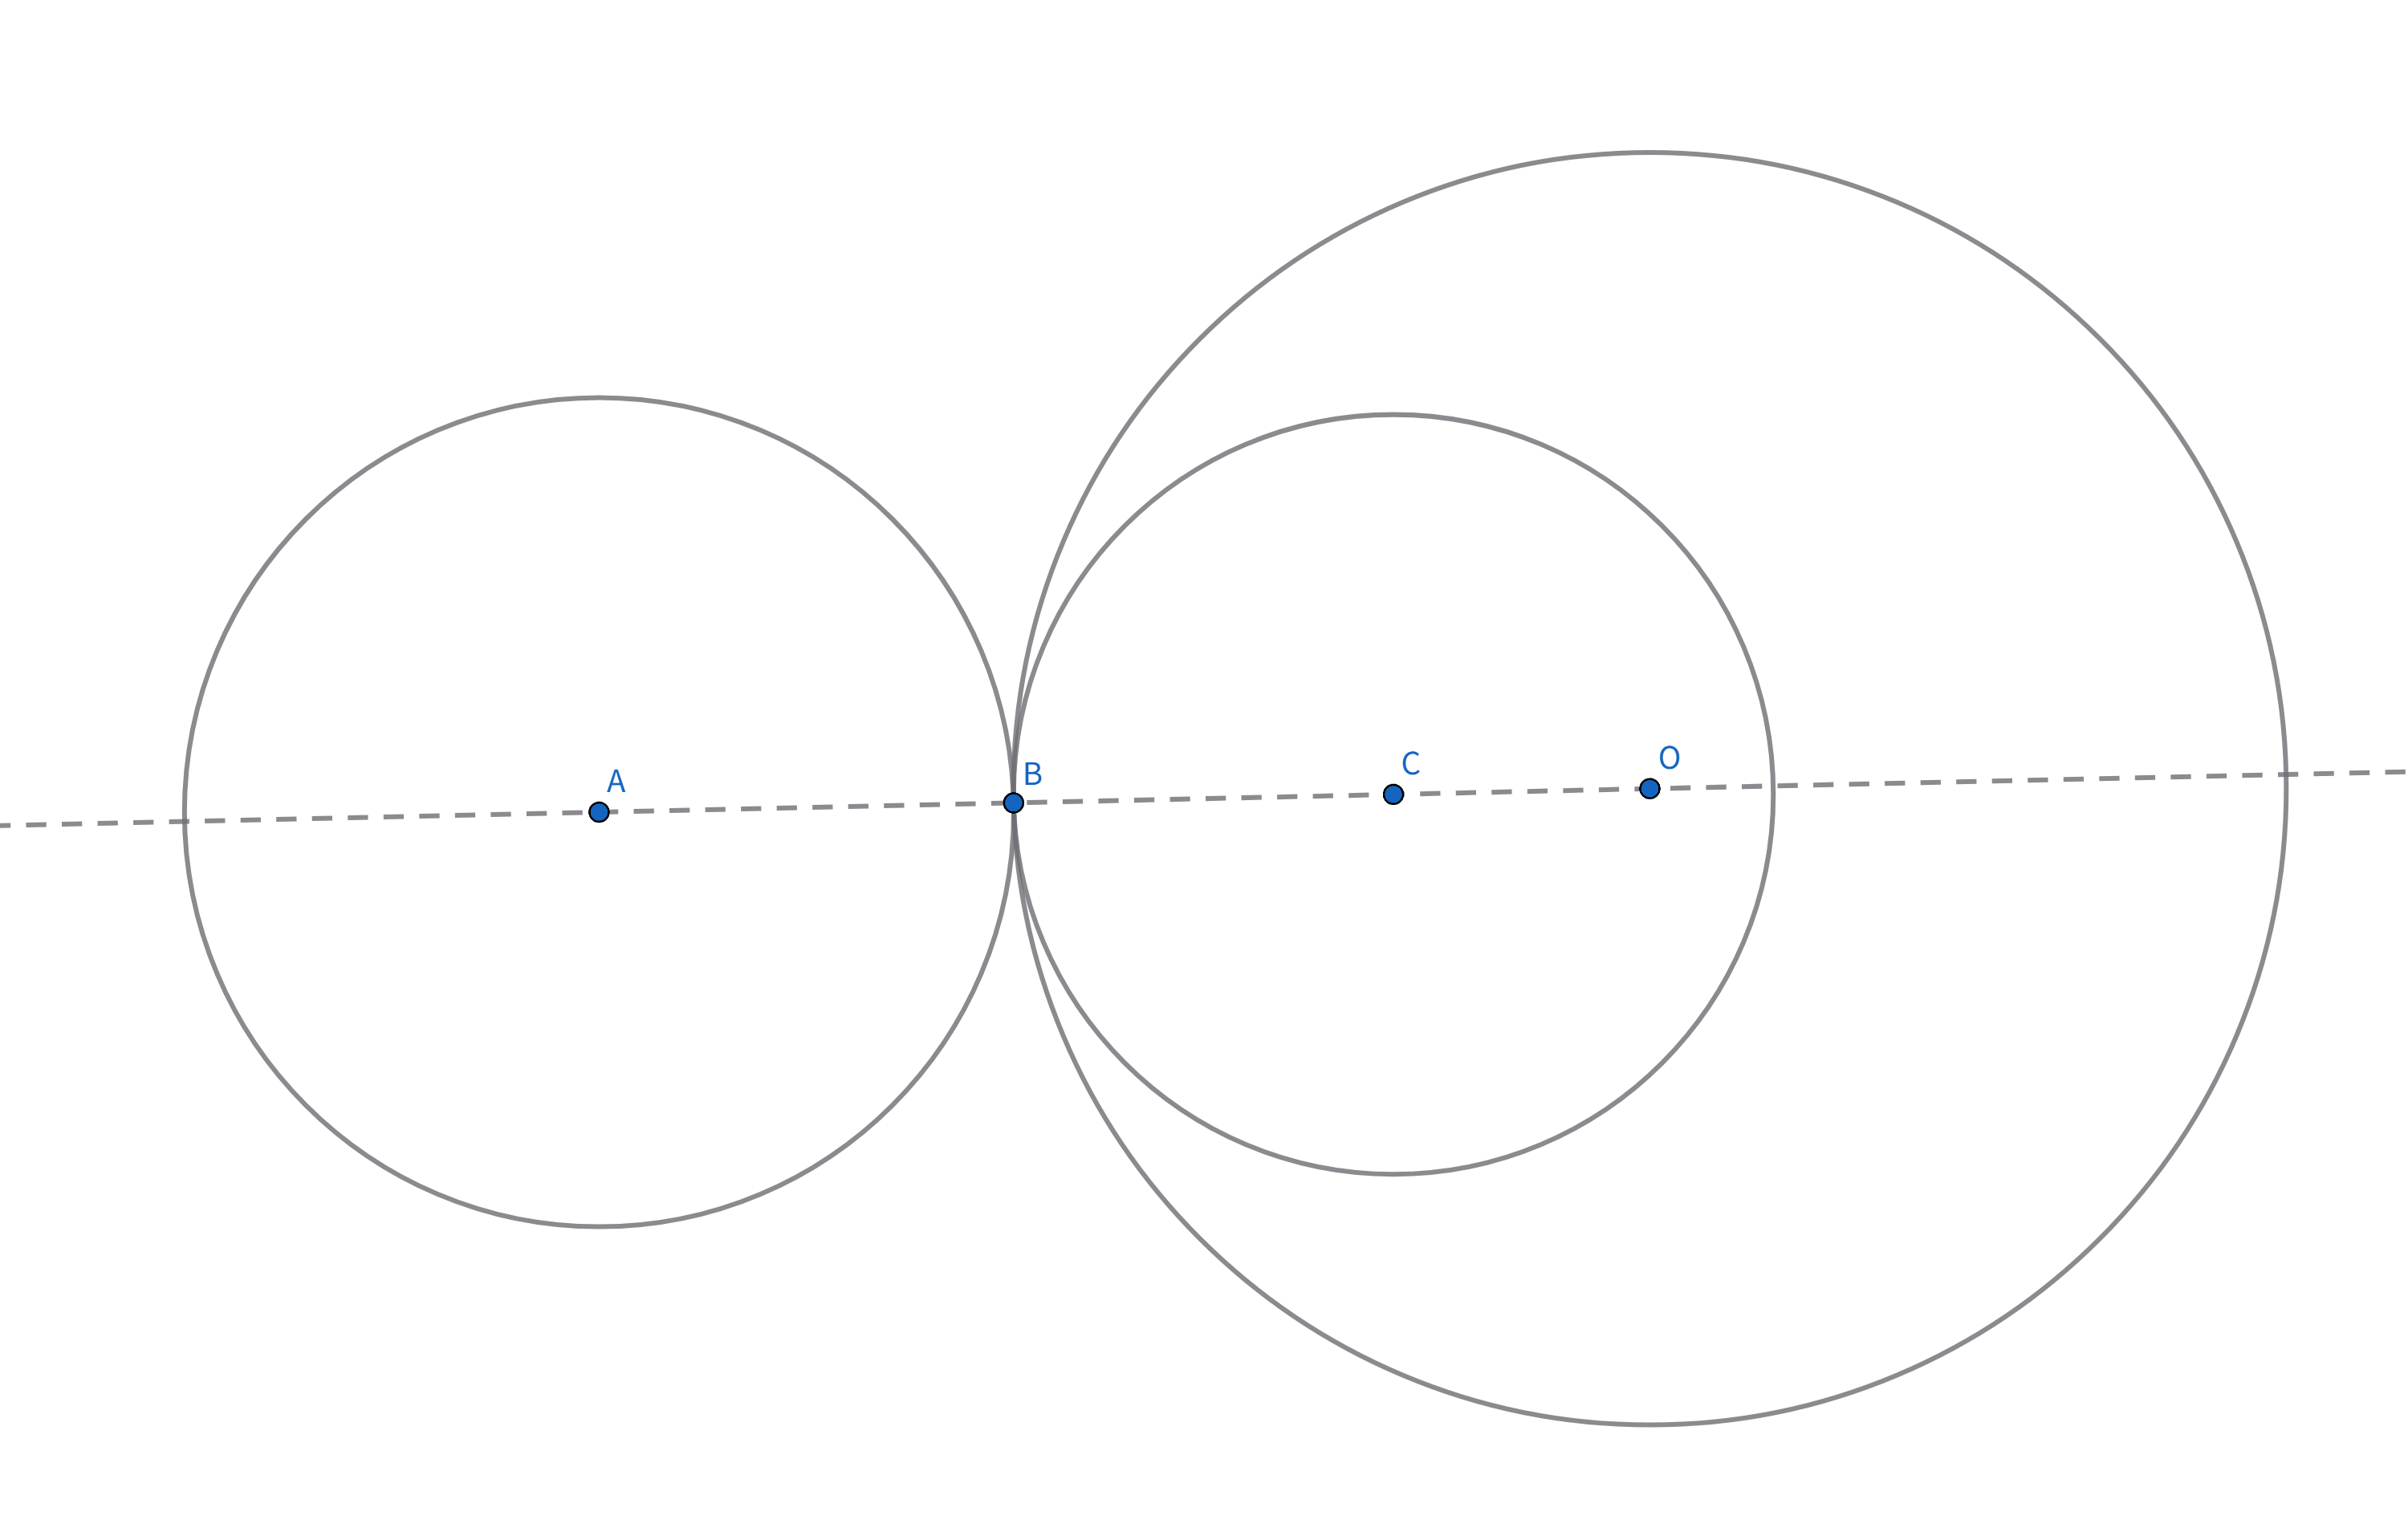
\includegraphics[width=0.5\linewidth]{figures/外切与内切.png}
    \caption{外切与内切}
    % \label{fig:enter-label}
\end{figure}
\begin{figure}[H]
    \centering
    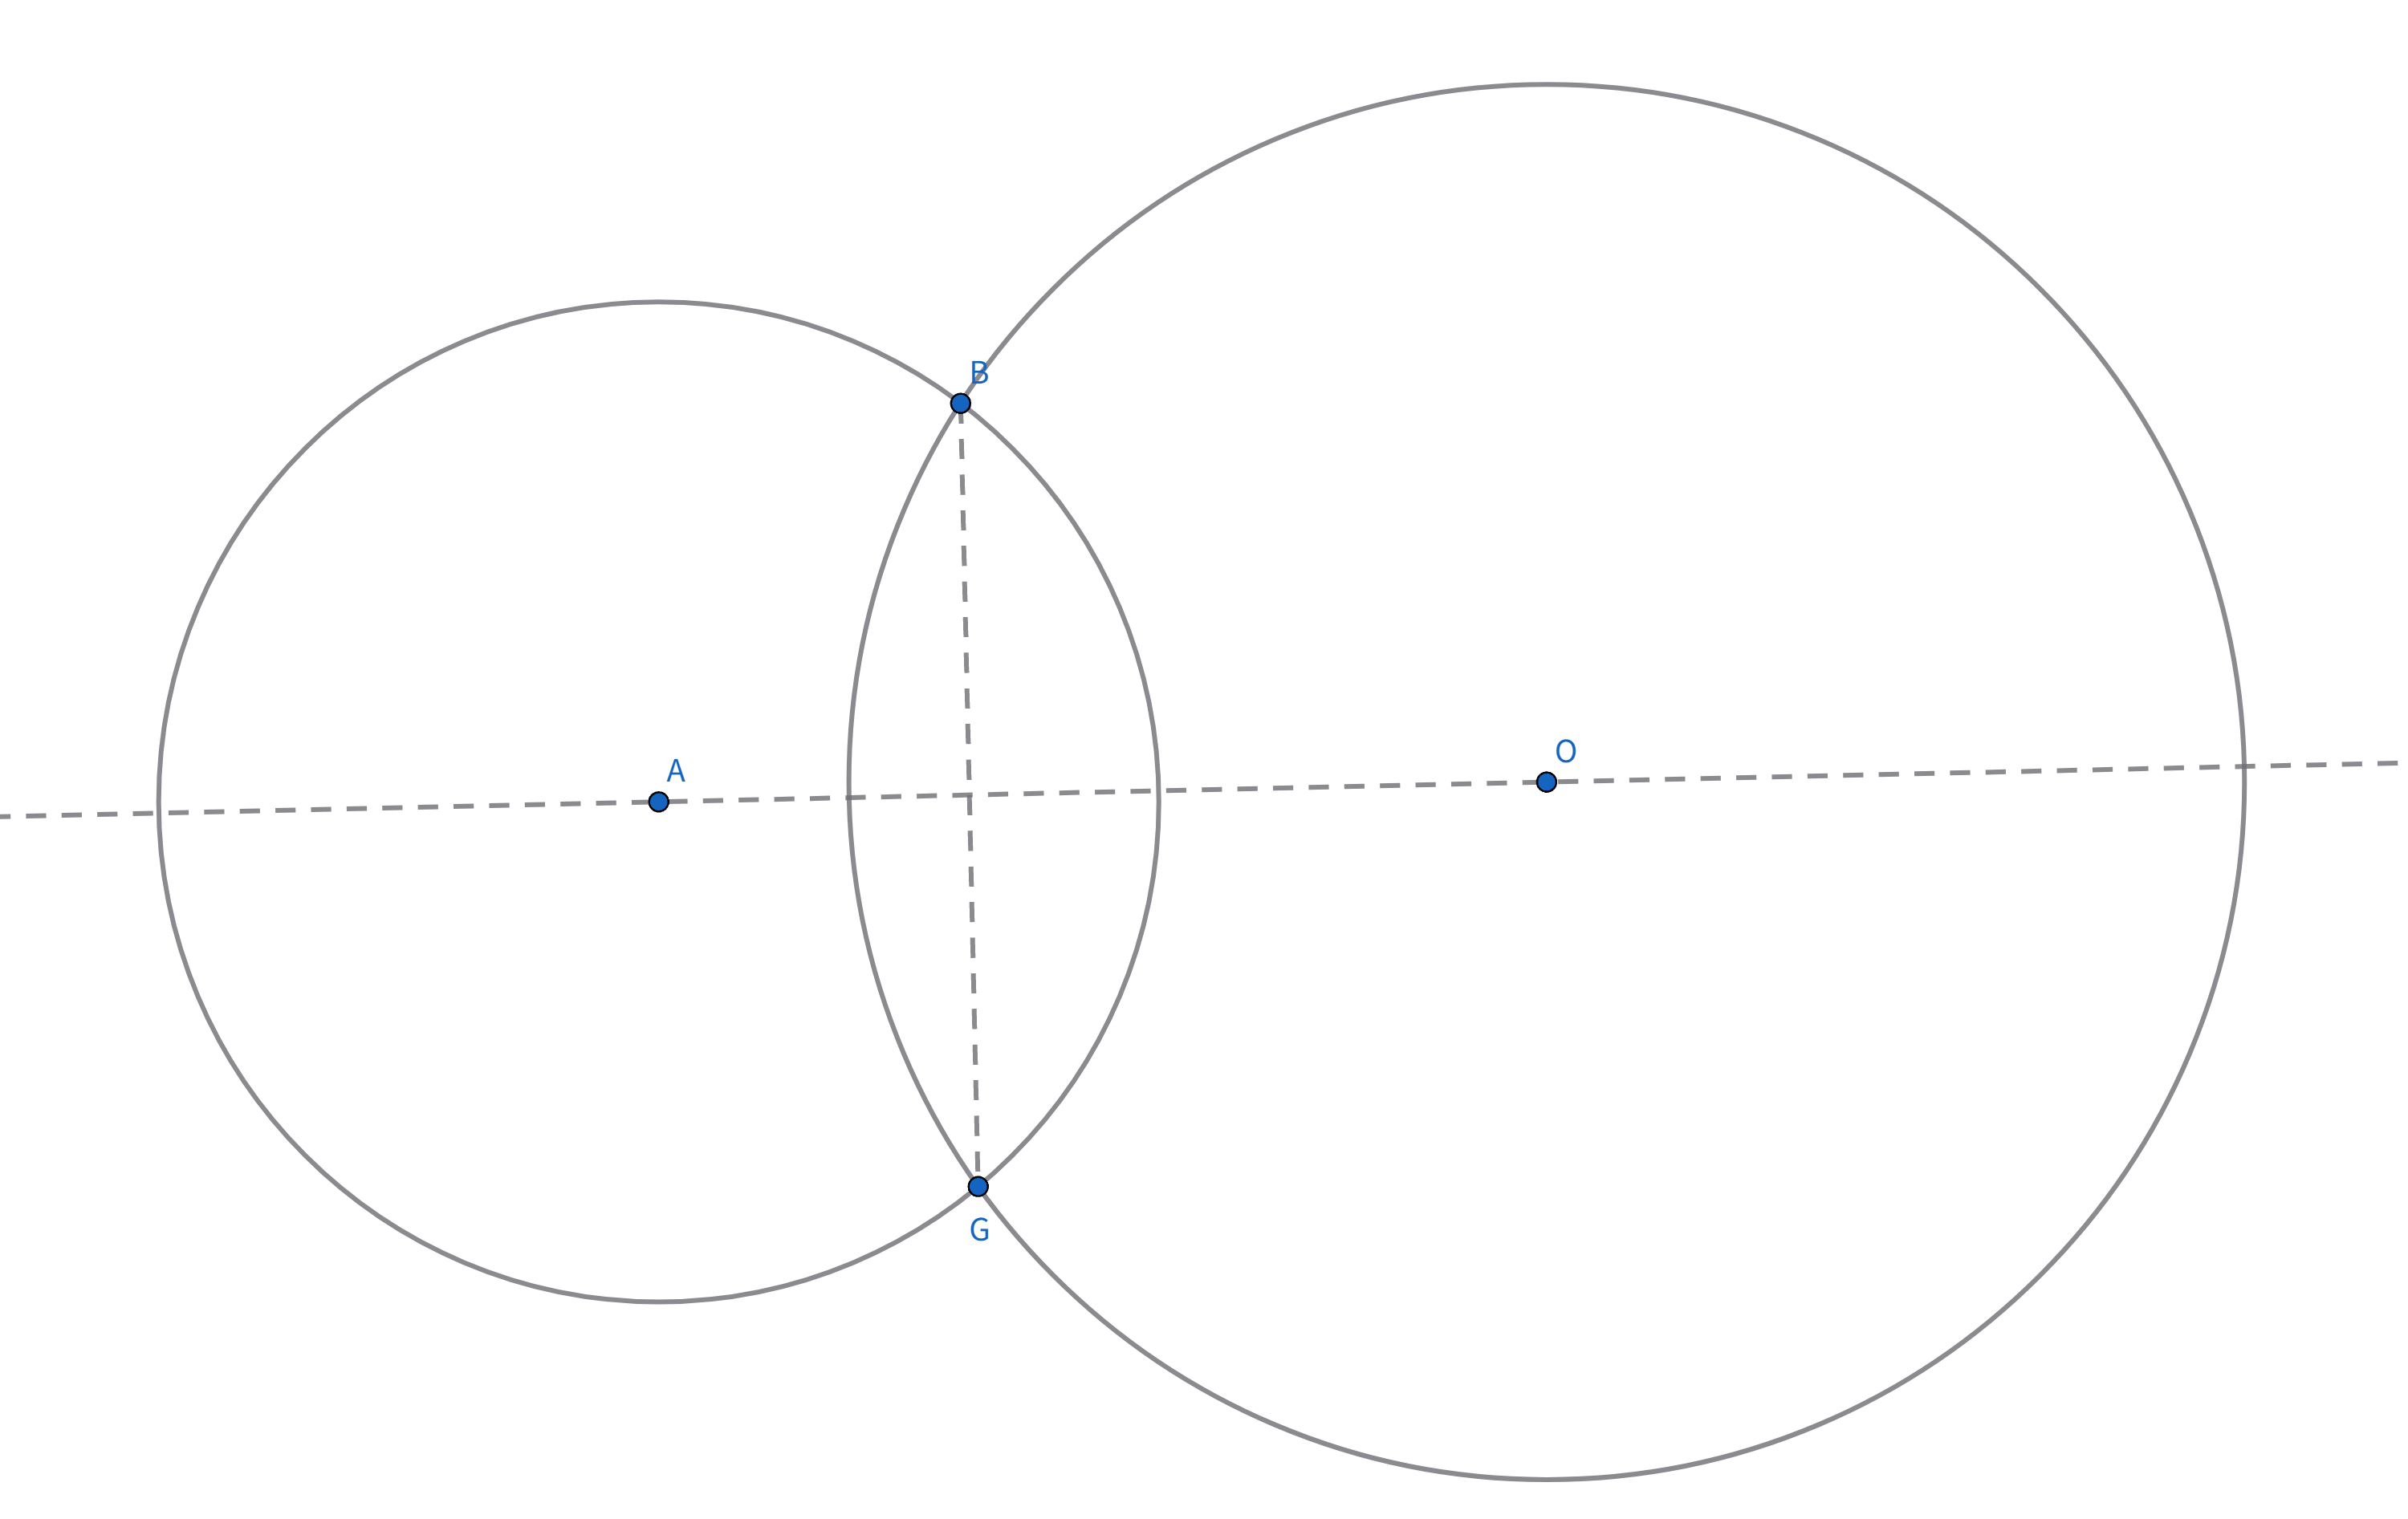
\includegraphics[width=0.5\linewidth]{figures/圆相交.png}
    \caption{圆相交}
    % \label{fig:enter-label}
\end{figure}



\section{外接圆}
\begin{definition}
任意不共线的三点A、B、C可以唯一确定一个圆,这个圆O称作是$\triangle ABC$的外接圆。

取三边BC、AB、AC的中点D、E、F,假设BC中垂线与AC中垂线交于O,则A、B、C三点一定在以O为圆心,以OA为半径的圆上。    
\end{definition}

\begin{theorem}
    对任意 $\triangle ABC$,一定有下式成立:
    $$\frac{BC}{\sin A} = \frac{AC}{\sin B} = \frac{AB}{\sin C}=2R.$$
\end{theorem}
\begin{figure}[H]
    \centering
    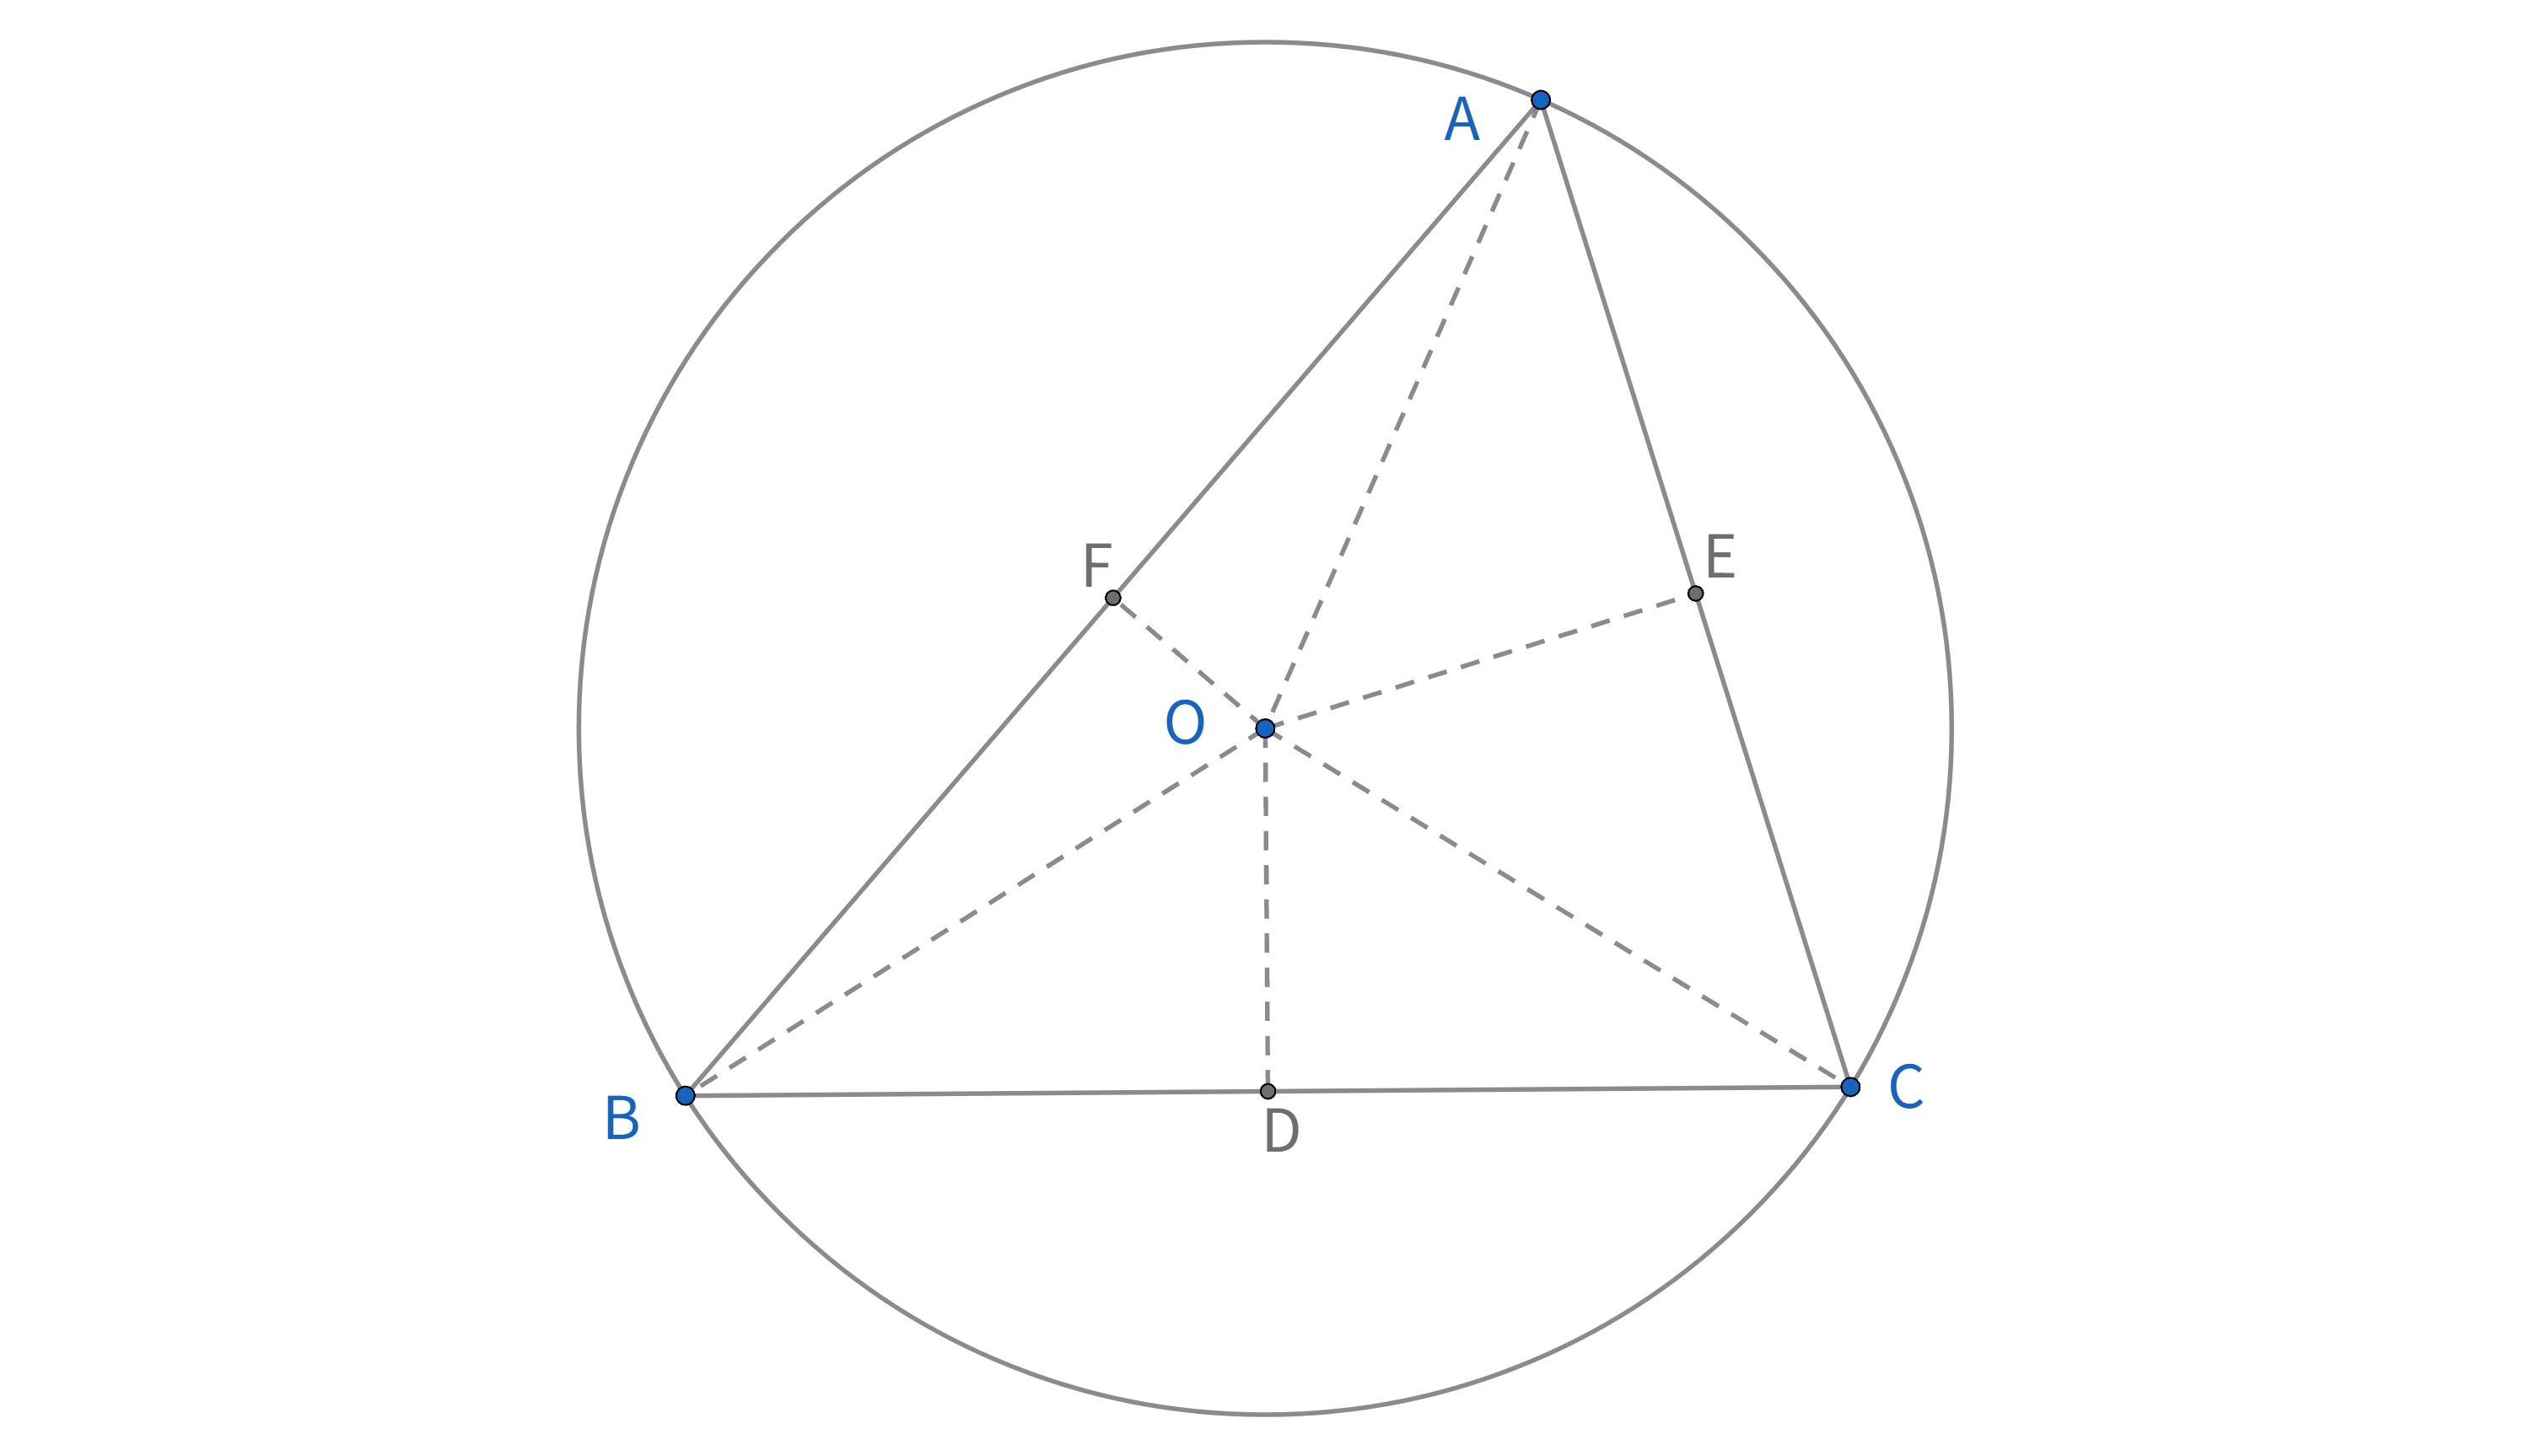
\includegraphics[width=\linewidth]{figures/正弦定理.png}
    \caption{正弦定理}
\end{figure}



